\section*{Supplementary data}

\setcounter{figure}{0}
\setcounter{table}{0}

\captionsetup[figure]{name=Supplementary Fig. S}
\captionsetup[table]{name=Supplementary Table S}

\begin{table}[h!]
\caption{
  {\bf Optimal cluster thresholds per pathogen, known genetic group type, and embedding method based on normalized variation of information (VI) distances calculated from early pathogen datasets.}
  Smaller VI values indicate fewer differences between HDBSCAN clusters and known genetic groups.
  VI of 0 indicates identical clusters and 1 indicates maximally different clusters.
  Threshold refers to the minimum Euclidean distance between initial clusters for HDBSCAN to consider them as distinct clusters.
  We apply these optimal thresholds per pathogen, known genetic group type, and method to find clusters in corresponding late datasets for each pathogen.}\label{S_Table_optimal_cluster_parameters}
\begin{tabular}{llrr}
\toprule
                     Pathogen & Method &   VI &  Threshold \\
\midrule
               Influenza H3N2 &  t-SNE & 0.04 &        2.0 \\
                              &   UMAP & 0.08 &        1.0 \\
                              &    MDS & 0.10 &        3.5 \\
                              &    PCA & 0.19 &        0.5 \\
SARS-CoV-2 (Nextstrain clade) &  t-SNE & 0.07 &        1.0 \\
                              &    MDS & 0.15 &        0.0 \\
                              &   UMAP & 0.16 &        0.5 \\
                              &    PCA & 0.22 &        0.5 \\
           SARS-CoV-2 (Pango) &  t-SNE & 0.12 &        1.0 \\
                              &    MDS & 0.23 &        0.0 \\
                              &   UMAP & 0.25 &        0.5 \\
                              &    PCA & 0.31 &        0.5 \\
\bottomrule
\end{tabular}

\end{table}

\begin{table}
\caption{{\bf Number of clusters, transitions between clusters in the phylogeny, and excess transitions indicating non-monophyletic groups per pathogen and embedding.}
Embeddings without any excess transitions reflect monophyletic groups in the corresponding pathogen phylogeny.}\label{S_Table_monophyletic_clusters}
\end{table}

\begin{table}
\caption{{\bf Mutations observed per embedding cluster relative to a reference genome sequence for each pathogen.}
Each row reflects the alternate allele identified at a specific position of the given pathogen genome or gene sequence, the pathogen dataset, the embedding method, the number of clusters in the embedding with the observed mutation, and the list of distinct cluster labels with the mutation.
Mutations must have occurred in at least 10 samples of the given dataset with an allele frequency of at least 50\%.
Cluster-specific mutations appear in rows with a \emph{cluster\_count} value of 1.}\label{S_Table_mutations_per_cluster}
\end{table}

\begin{table}
\caption{{\bf Average Euclidean distances between each known recombinant, $X$, and its parental lineages $A$ and $B$ per embedding method.}
Distances include average pairwise comparisons between $A$ and $B$, $A$ and $X$, and $B$ and $X$.
Additional columns indicate whether each recombinant lineage maps closer to both parental lineages (or at least one) than those parents map to each other.}\label{S_Table_recombinant_distances}
\end{table}

\begin{table}
\caption{{\bf Accessions and authors from originating and submitting laboratories of seasonal influenza and SARS-CoV-2 sequences from INSDC databases.}}\label{S_Table_accessions}
\end{table}

\begin{figure}[!h]
  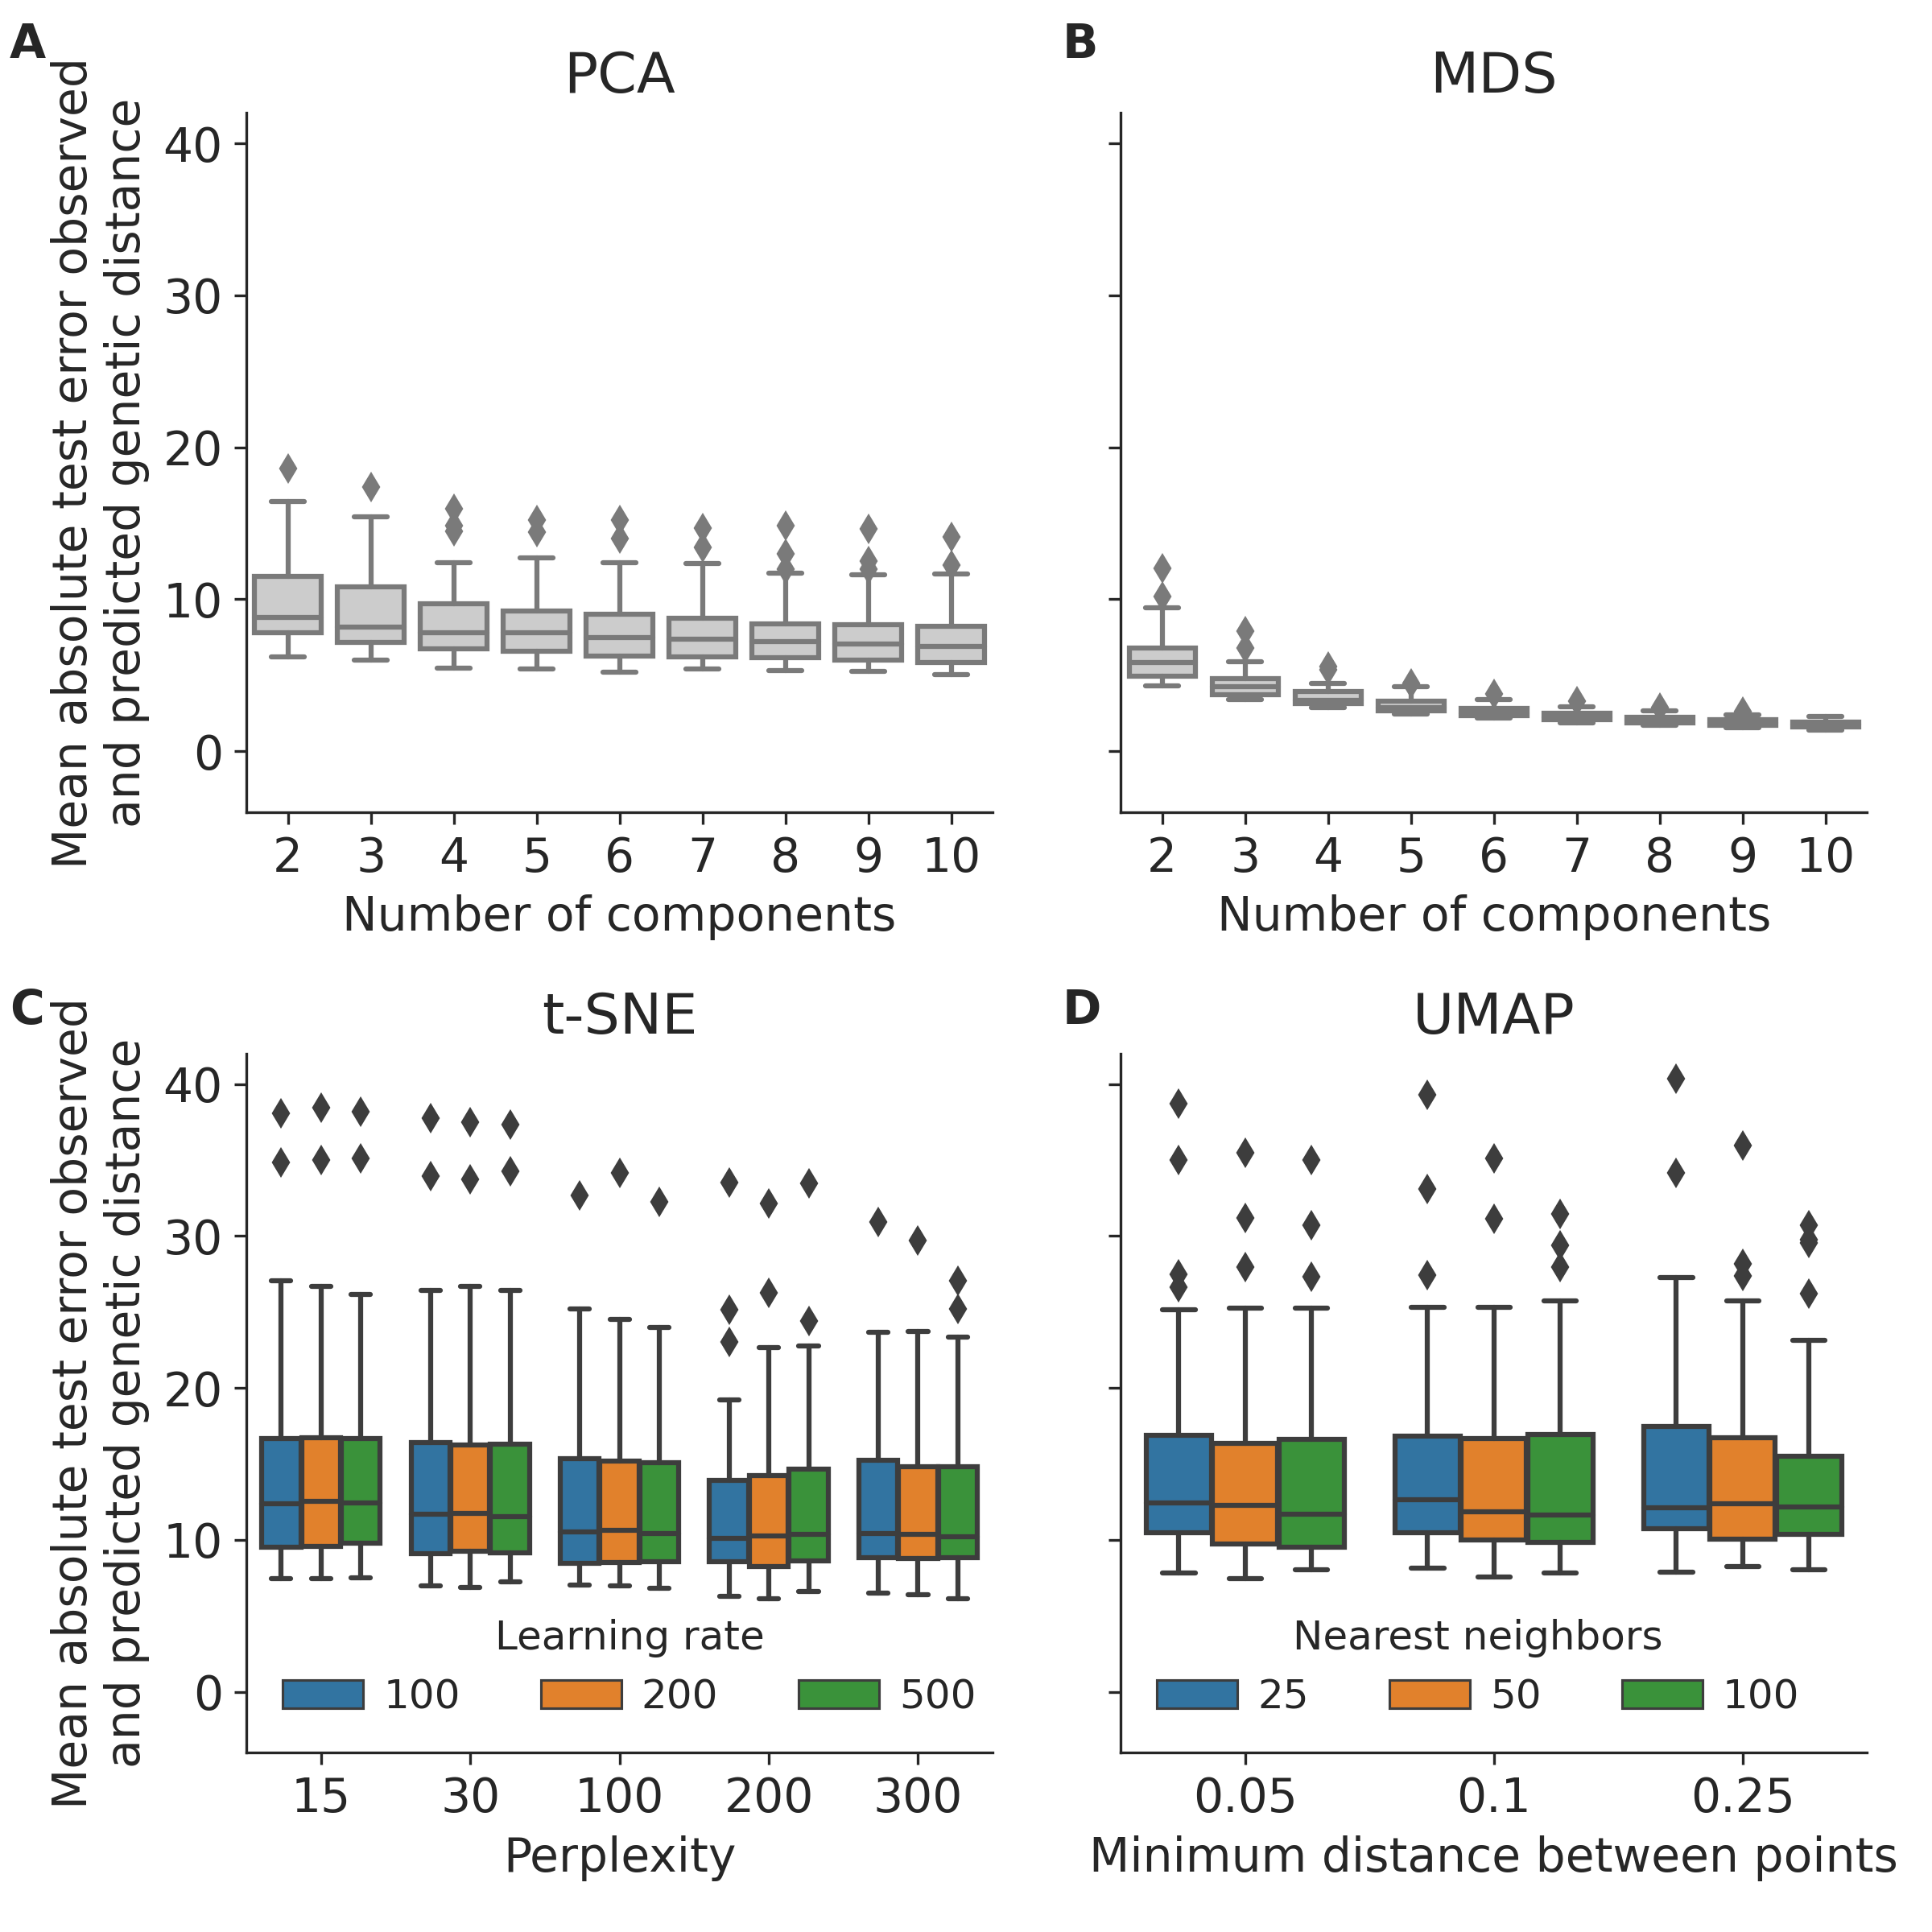
\includegraphics[width=0.9\columnwidth]{figures/simulated-influenza-like-with-no-reassortment-scores-by-parameters.png}
  \caption{{\bf Distribution of mean absolute errors (MAE) between observed and predicted pairwise genetic distances per embedding method parameters for simulated influenza-like populations.}}\label{S_Fig_simulated_flu_errors}
\end{figure}

\begin{figure}[!h]
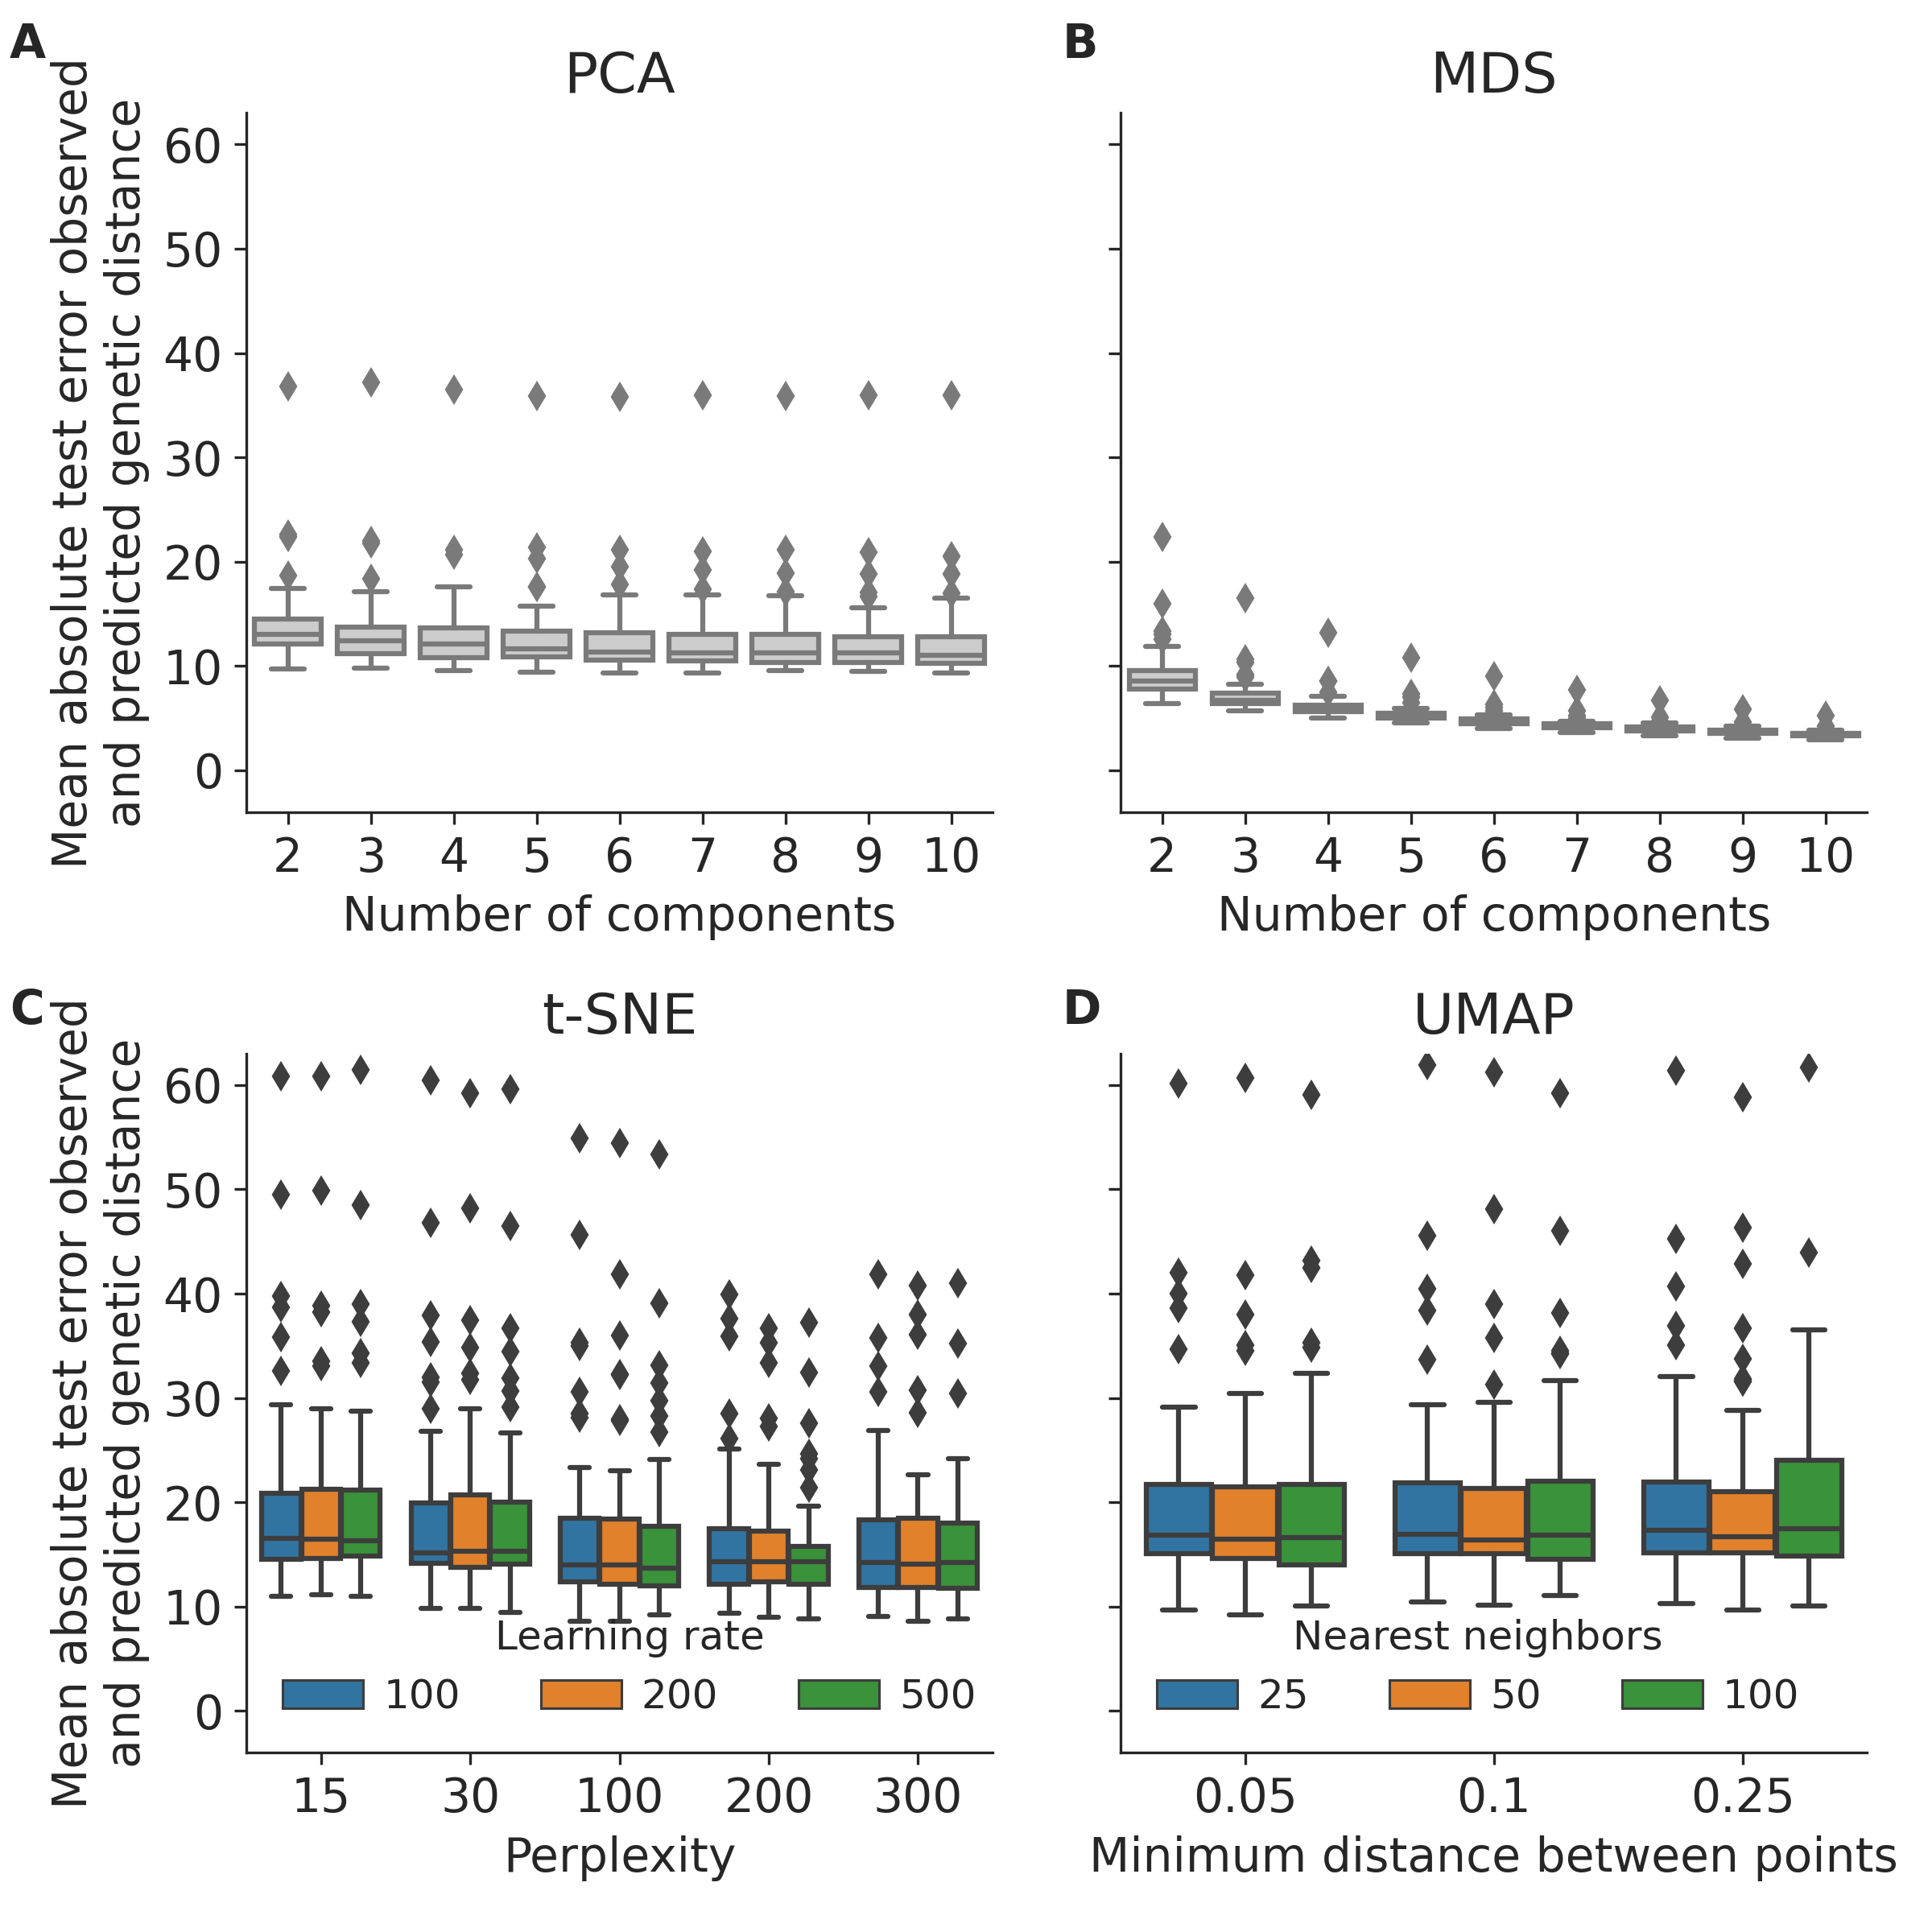
\includegraphics[width=\columnwidth]{figures/simulated-coronavirus-like-with-moderate-recombination-rate-scores-by-parameters.png}
\caption{{\bf Distribution of mean absolute errors (MAE) between observed and predicted pairwise genetic distances per embedding method parameters for simulated coronavirus-like populations.}}\label{S_Fig_simulated_coronavirus_errors}
\end{figure}

\begin{figure}[!h]
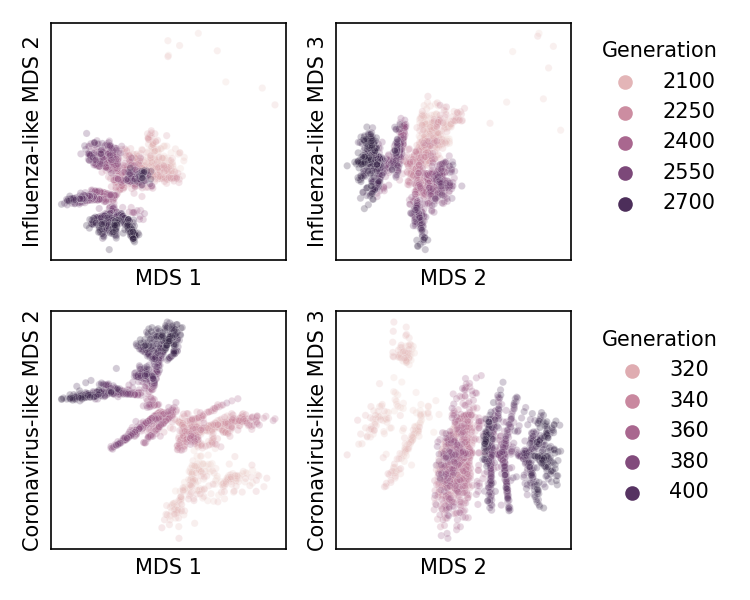
\includegraphics[width=\columnwidth]{figures/simulated-populations-representative-mds-embeddings.png}
\caption{{\bf Representative MDS embeddings for simulated populations using optimal parameters per pathogen (rows) and showing all three components.}}\label{S_Fig_simulated_representative_mds_embeddings}
\end{figure}

\begin{figure}[!h]
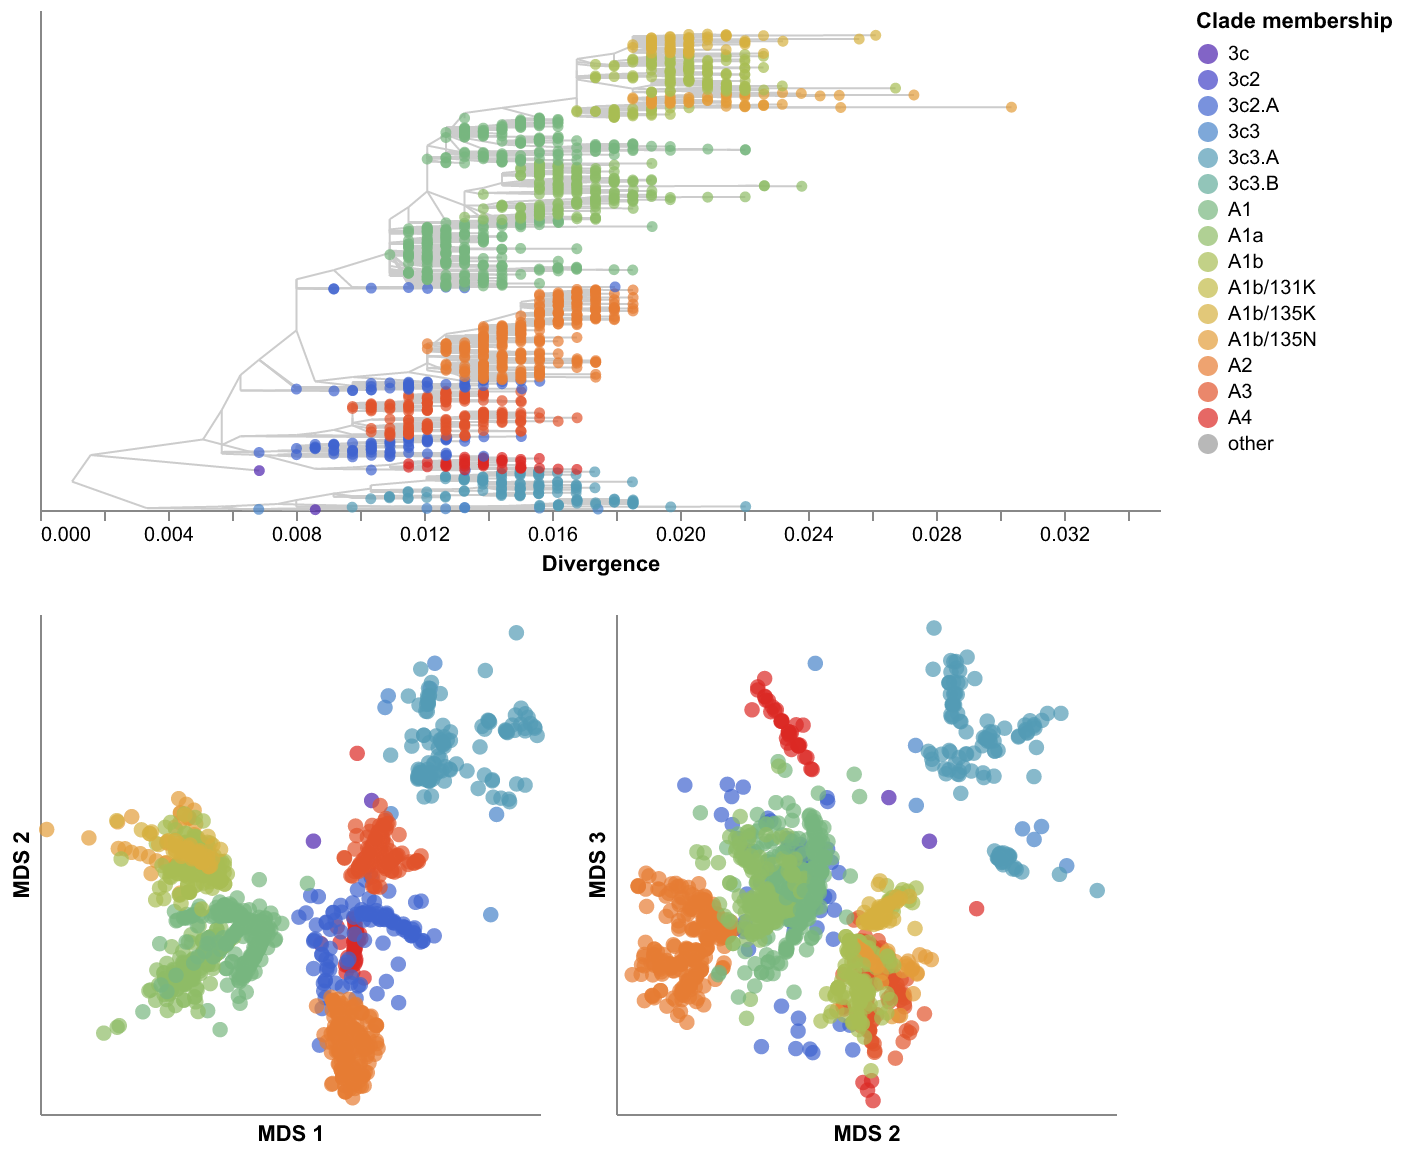
\includegraphics[width=\columnwidth]{figures/flu-2016-2018-mds-by-clade.png}
\caption{{\bf MDS embeddings for early (2016--2018) influenza H3N2 HA sequences showing all three components.}
Line segments in each embedding reflect phylogenetic relationships with internal node positions calculated from the mean positions of their immediate descendants in each dimension (see Methods).
Line colors represent the clade membership of the most ancestral node in the pair of nodes connected by the segment.
Line thickness scales by the square root of the number of leaves descending from a given node in the phylogeny.}\label{S_Fig_early_flu_mds_embeddings}
\end{figure}

\begin{figure}[!h]
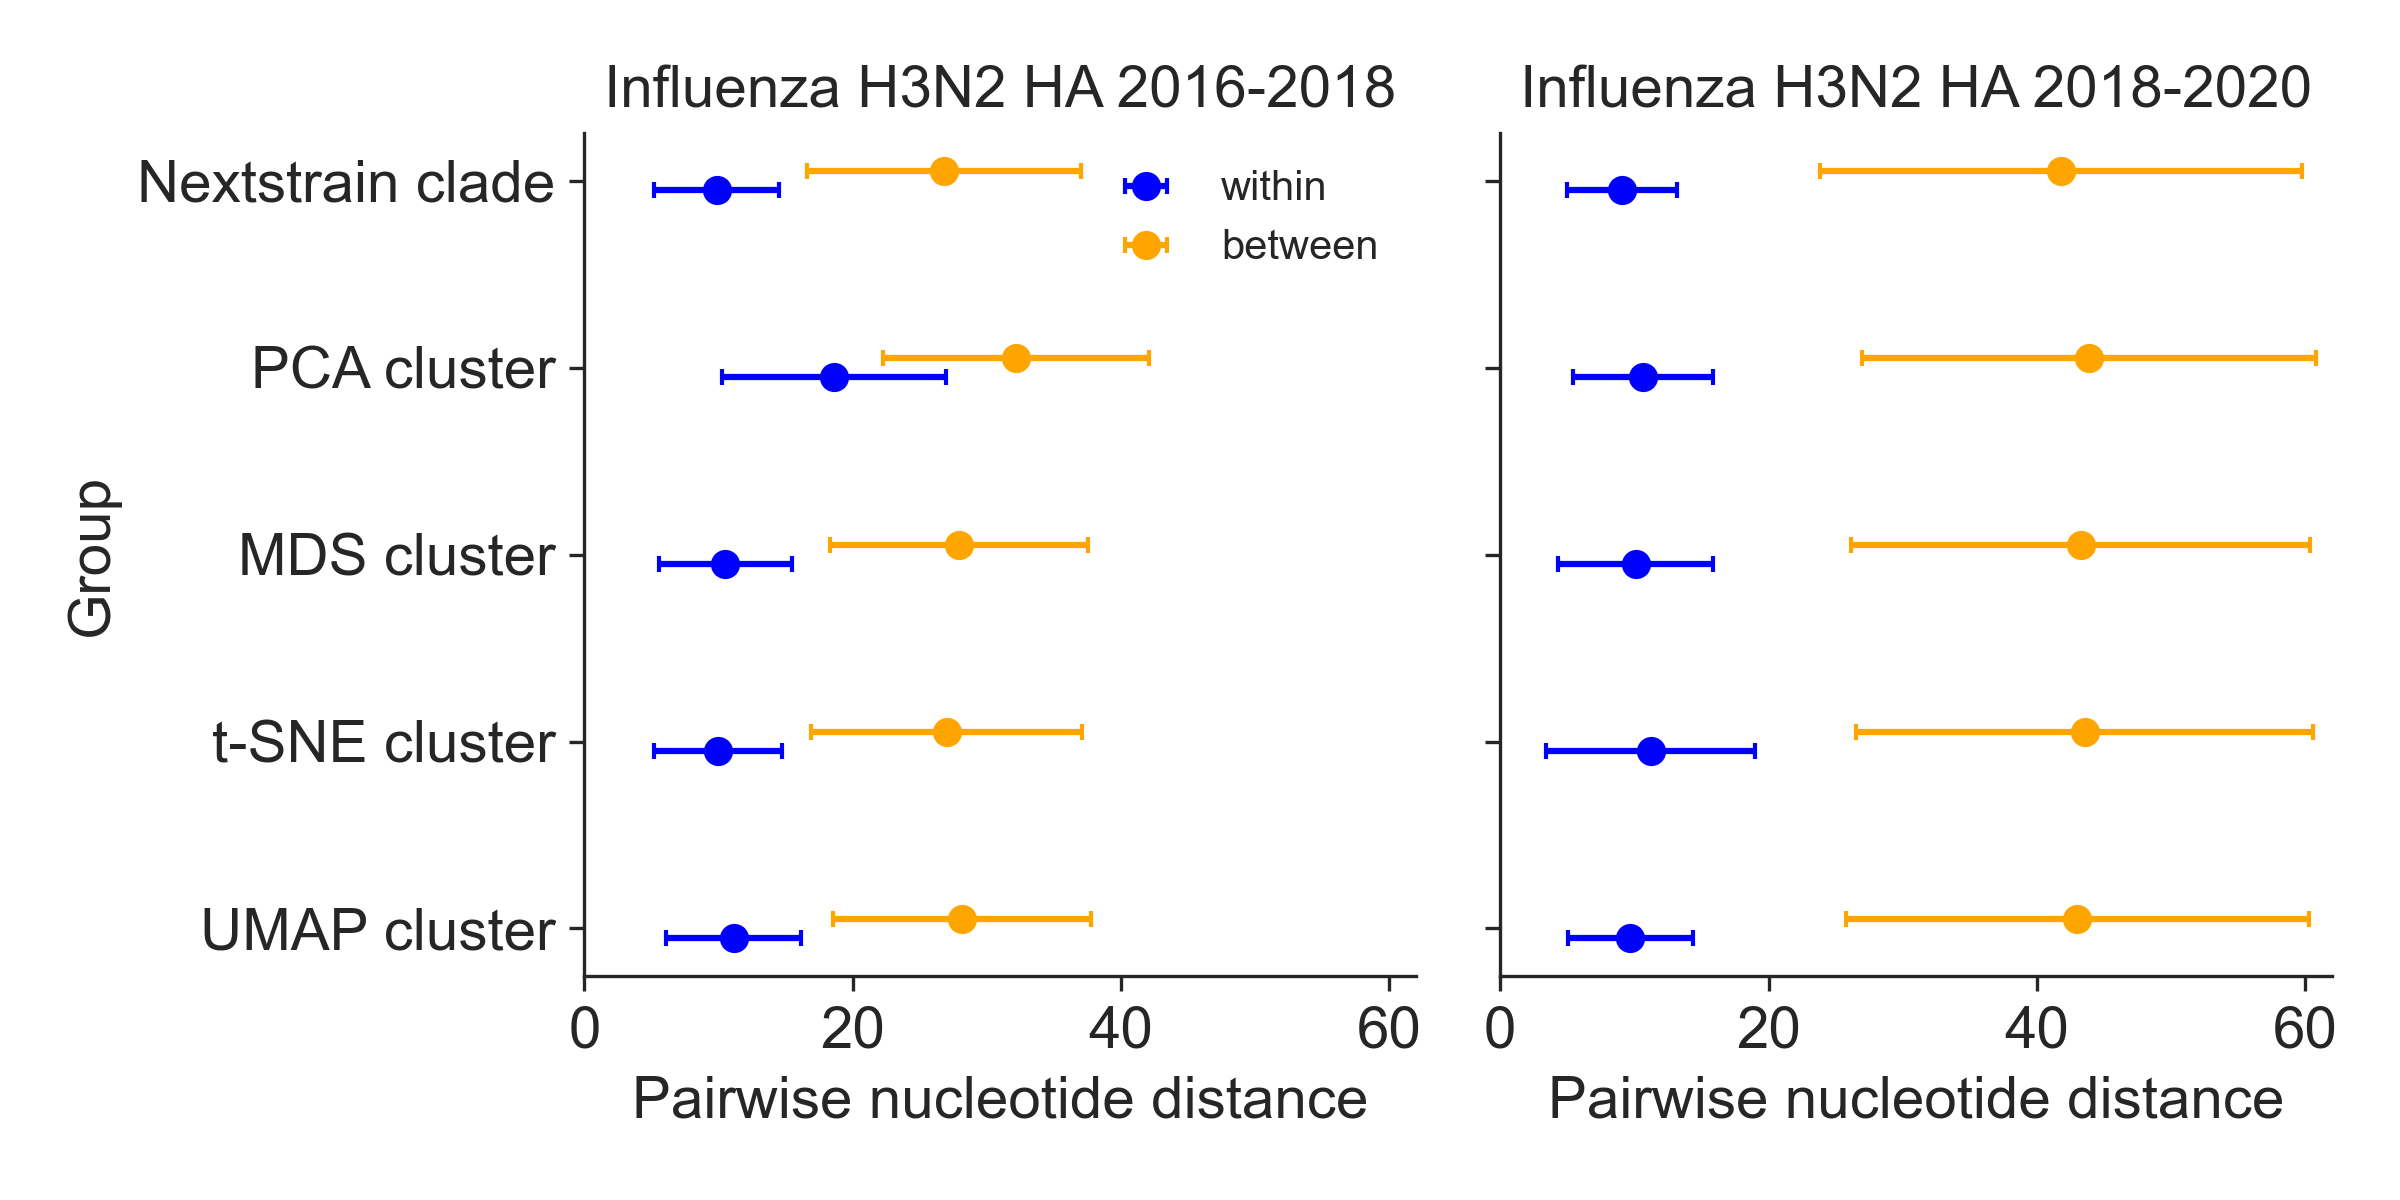
\includegraphics[width=\columnwidth]{figures/within_between_influenza.png}
\caption{{\bf Pairwise nucleotide distances for early (2016--2018) and late (2018--2020) influenza H3N2 HA sequences within and between genetic groups defined by Nextstrain clades and clusters from PCA, MDS, t-SNE, and UMAP embeddings.}}\label{S_Fig_flu_within_between_group_distances}
\end{figure}

\begin{figure}[!h]
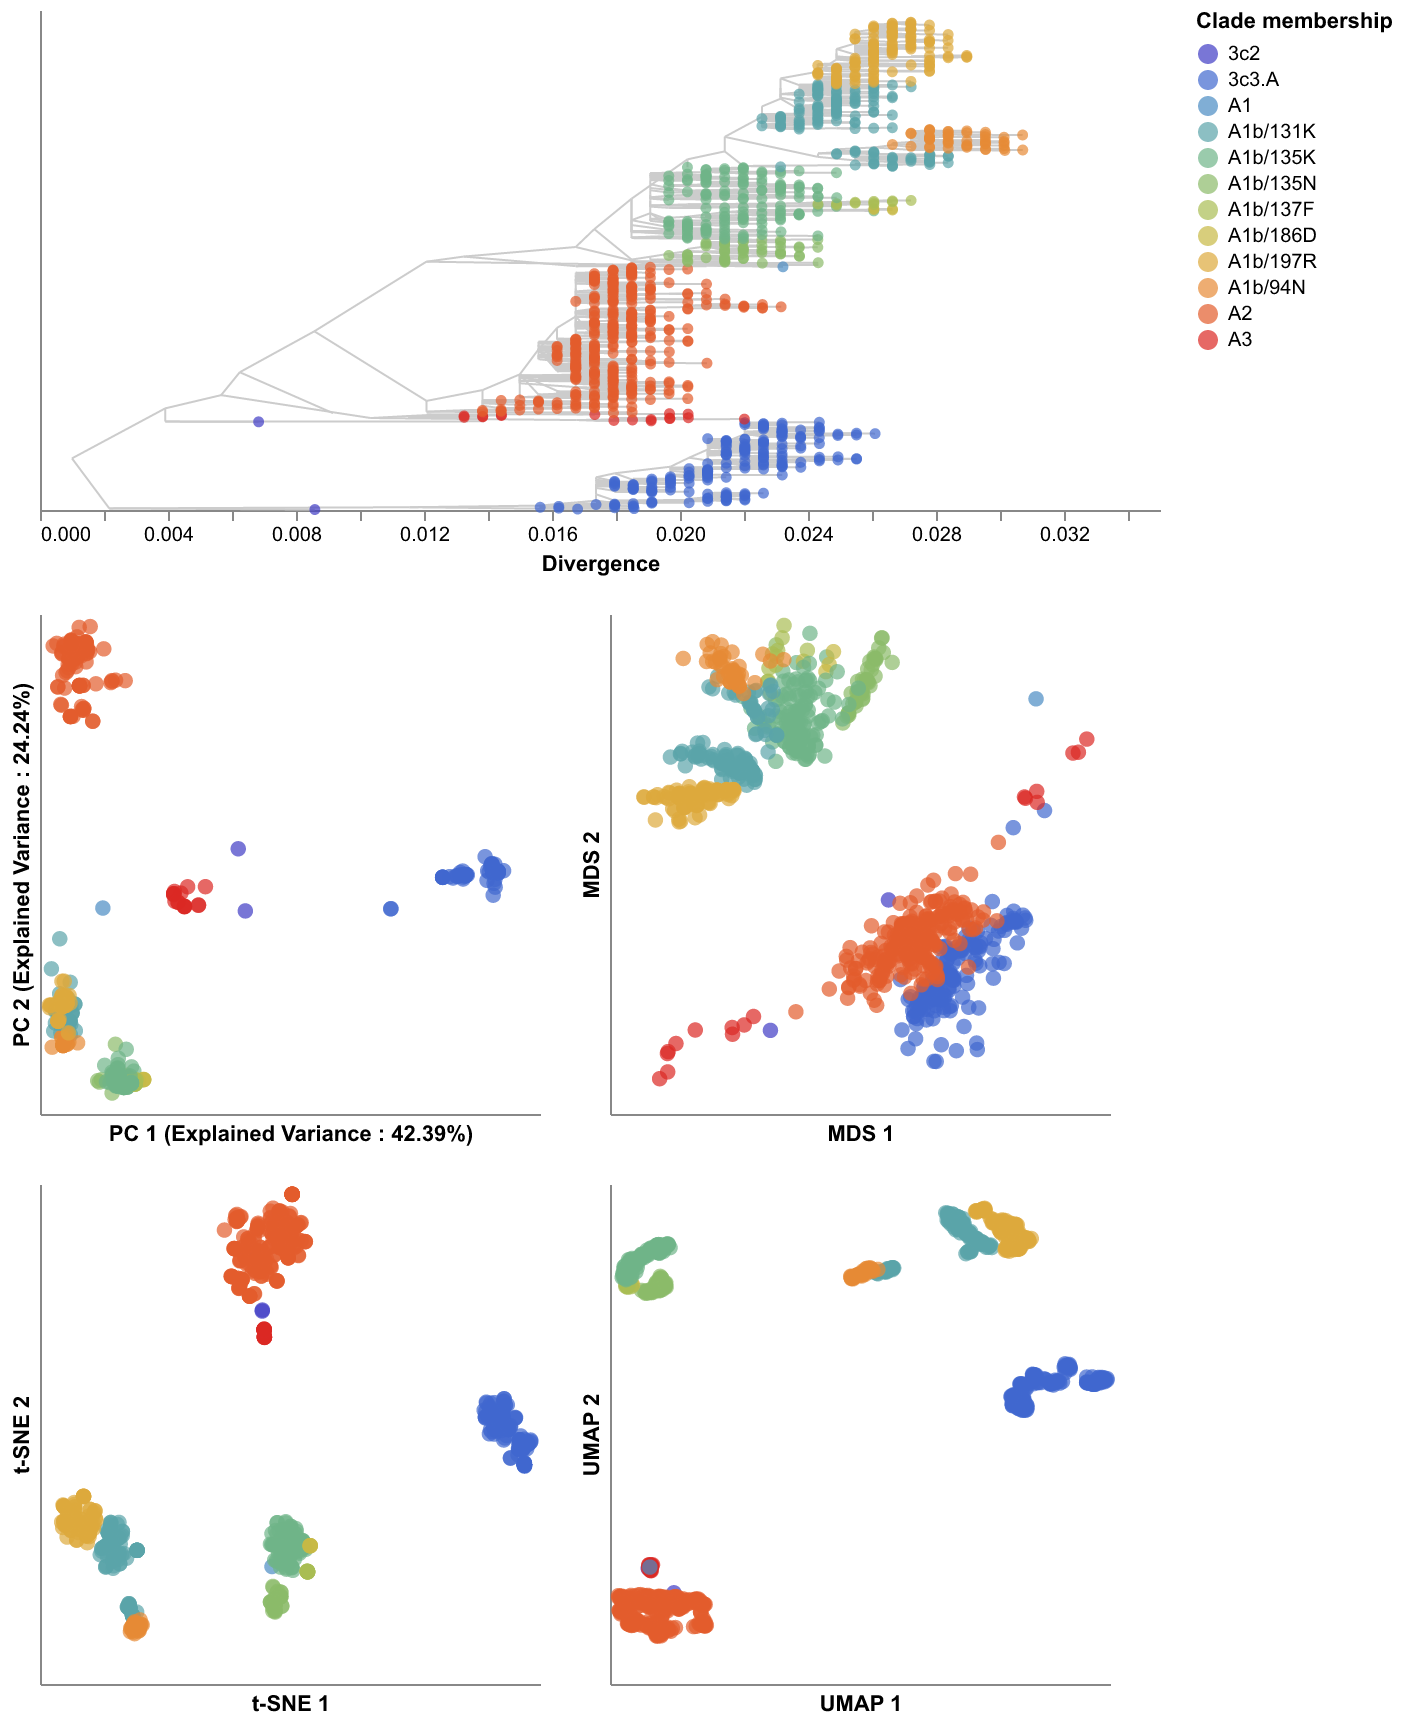
\includegraphics[width=\columnwidth]{figures/flu-2018-2020-ha-embeddings-by-clade.png}
\caption{{\bf Phylogeny of late (2018--2020) influenza H3N2 HA sequences plotted by nucleotide substitutions per site on the x-axis (top) and low-dimensional embeddings of the same sequences by PCA (middle left), MDS (middle right), t-SNE (bottom left), and UMAP (bottom right).}
Tips in the tree and embeddings are colored by their Nextstrain clade assignment.
Line segments in each embedding reflect phylogenetic relationships with internal node positions calculated from the mean positions of their immediate descendants in each dimension (see Methods).
Line colors represent the clade membership of the most ancestral node in the pair of nodes connected by the segment.
Line thickness scales by the square root of the number of leaves descending from a given node in the phylogeny.}\label{S_Fig_late_flu_embeddings_by_clade}
\end{figure}

\begin{figure}[!h]
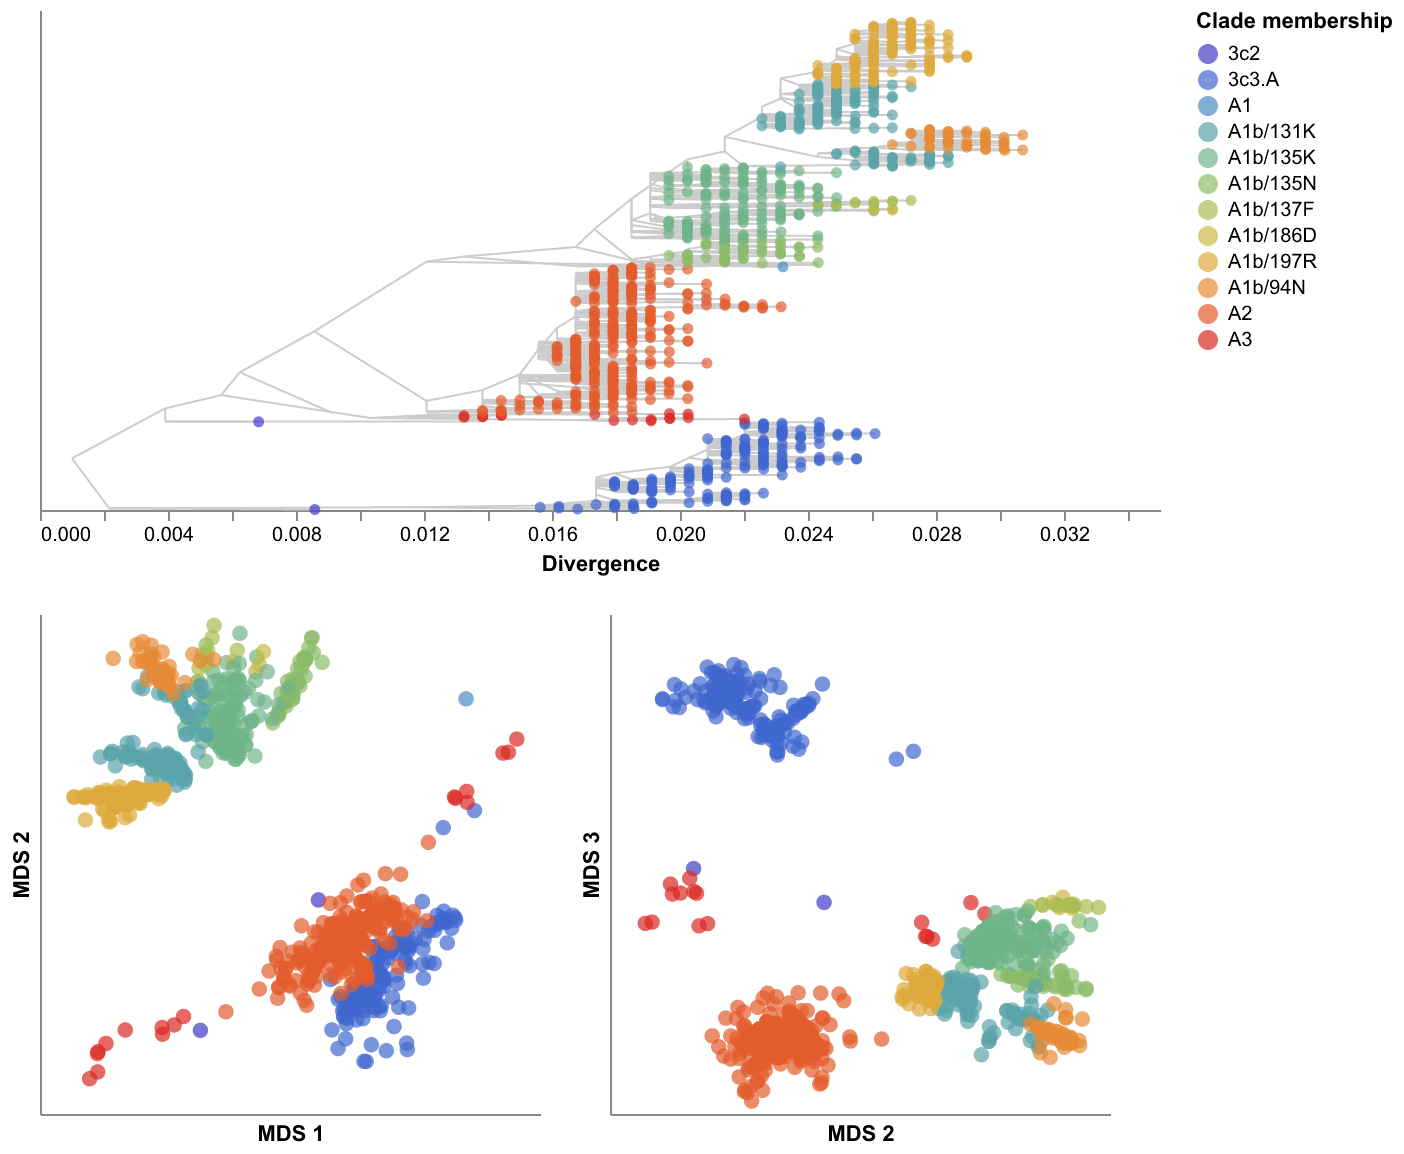
\includegraphics[width=\columnwidth]{figures/flu-2018-2020-mds-by-clade.png}
\caption{{\bf MDS embeddings for late (2018--2020) influenza H3N2 HA sequences showing all three components.}
Line segments in each embedding reflect phylogenetic relationships with internal node positions calculated from the mean positions of their immediate descendants in each dimension (see Methods).
Line colors represent the clade membership of the most ancestral node in the pair of nodes connected by the segment.
Line thickness scales by the square root of the number of leaves descending from a given node in the phylogeny.}\label{S_Fig_late_flu_mds_embeddings}
\end{figure}

\begin{figure}[!h]
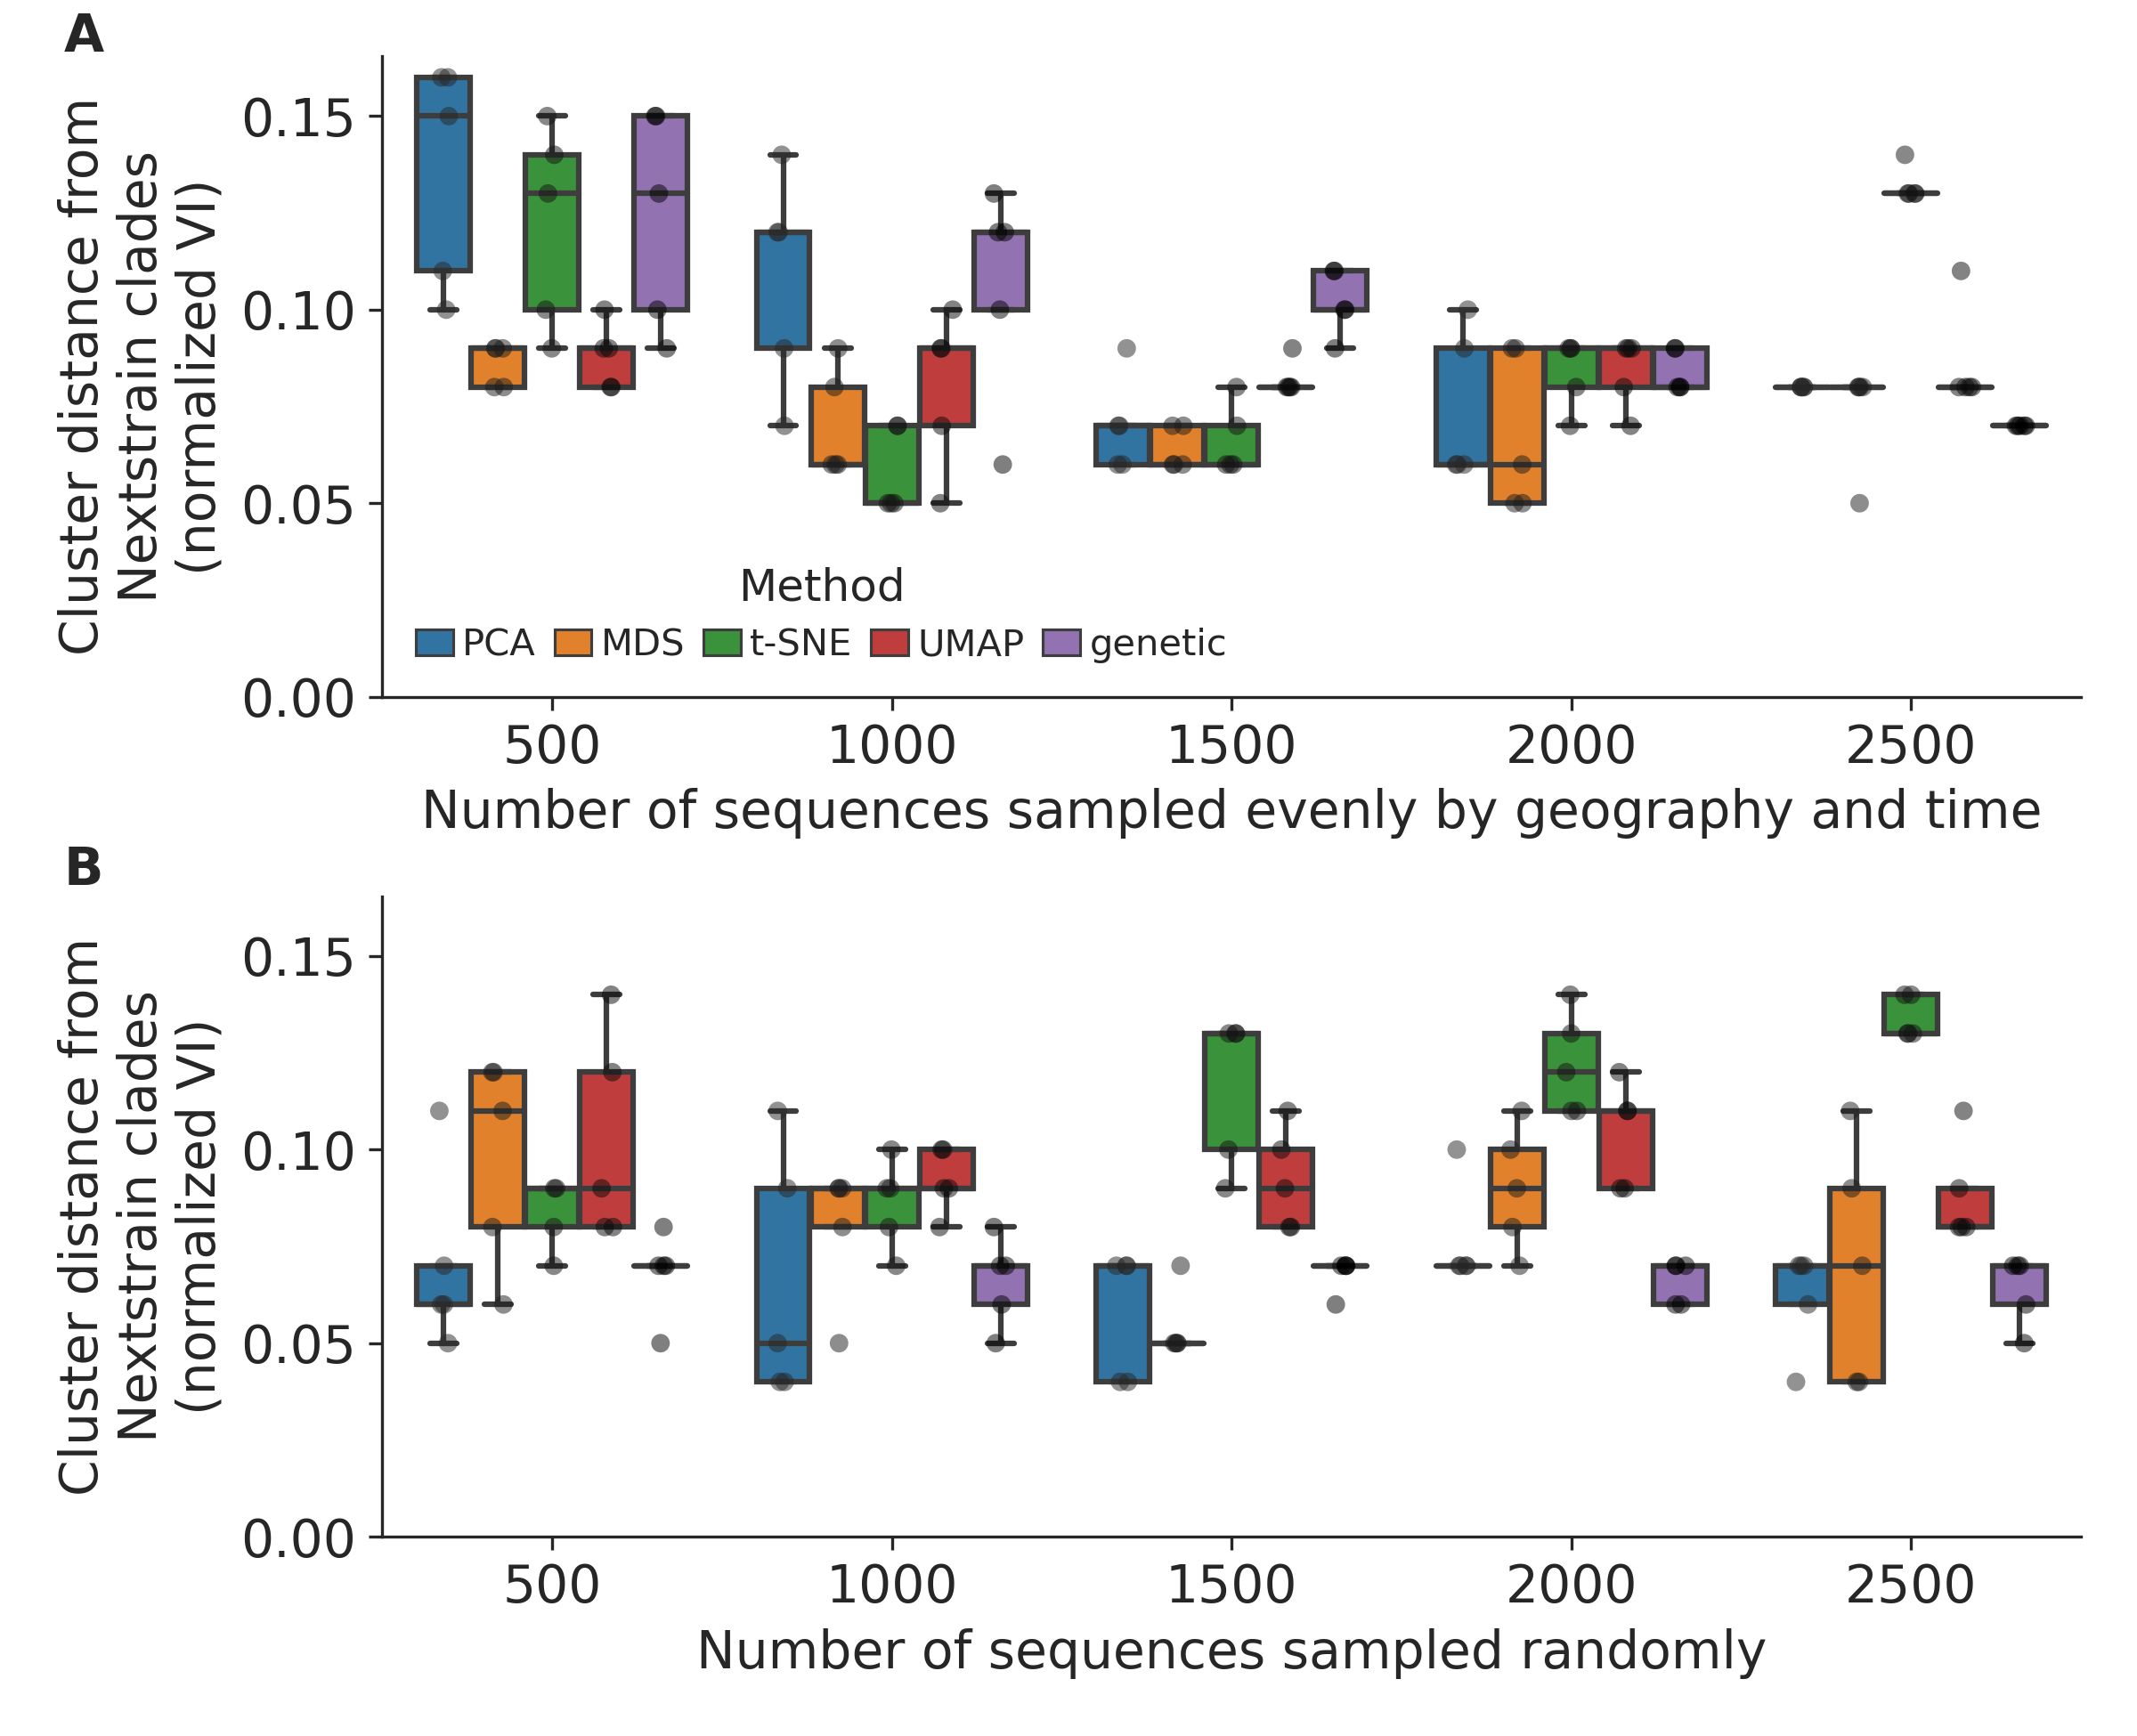
\includegraphics[width=\columnwidth]{figures/flu-2018-2020-replication-of-cluster-accuracy.png}
\caption{{\bf Replication of cluster accuracy per embedding method for late (2018--2020) influenza H3N2 HA sequences across different sampling densities (total sequences sampled) and sampling schemes including A) even geographic and temporal sampling and B) random sampling.}
  We measured cluster accuracy across five replicates per sampling density and scheme with the normalized VI distance between clusters from a given embedding and Nextstrain clades for the same samples.
  The even sampling scheme selected sequences evenly across country, year, and month to minimize geographic and temporal bias.
  The random sampling scheme uniformly sampled from the original dataset, reflecting the geographic and genetic bias in those data.}\label{S_Fig_late_flu_replication_of_cluster_accuracy}
\end{figure}

\begin{figure}[!h]
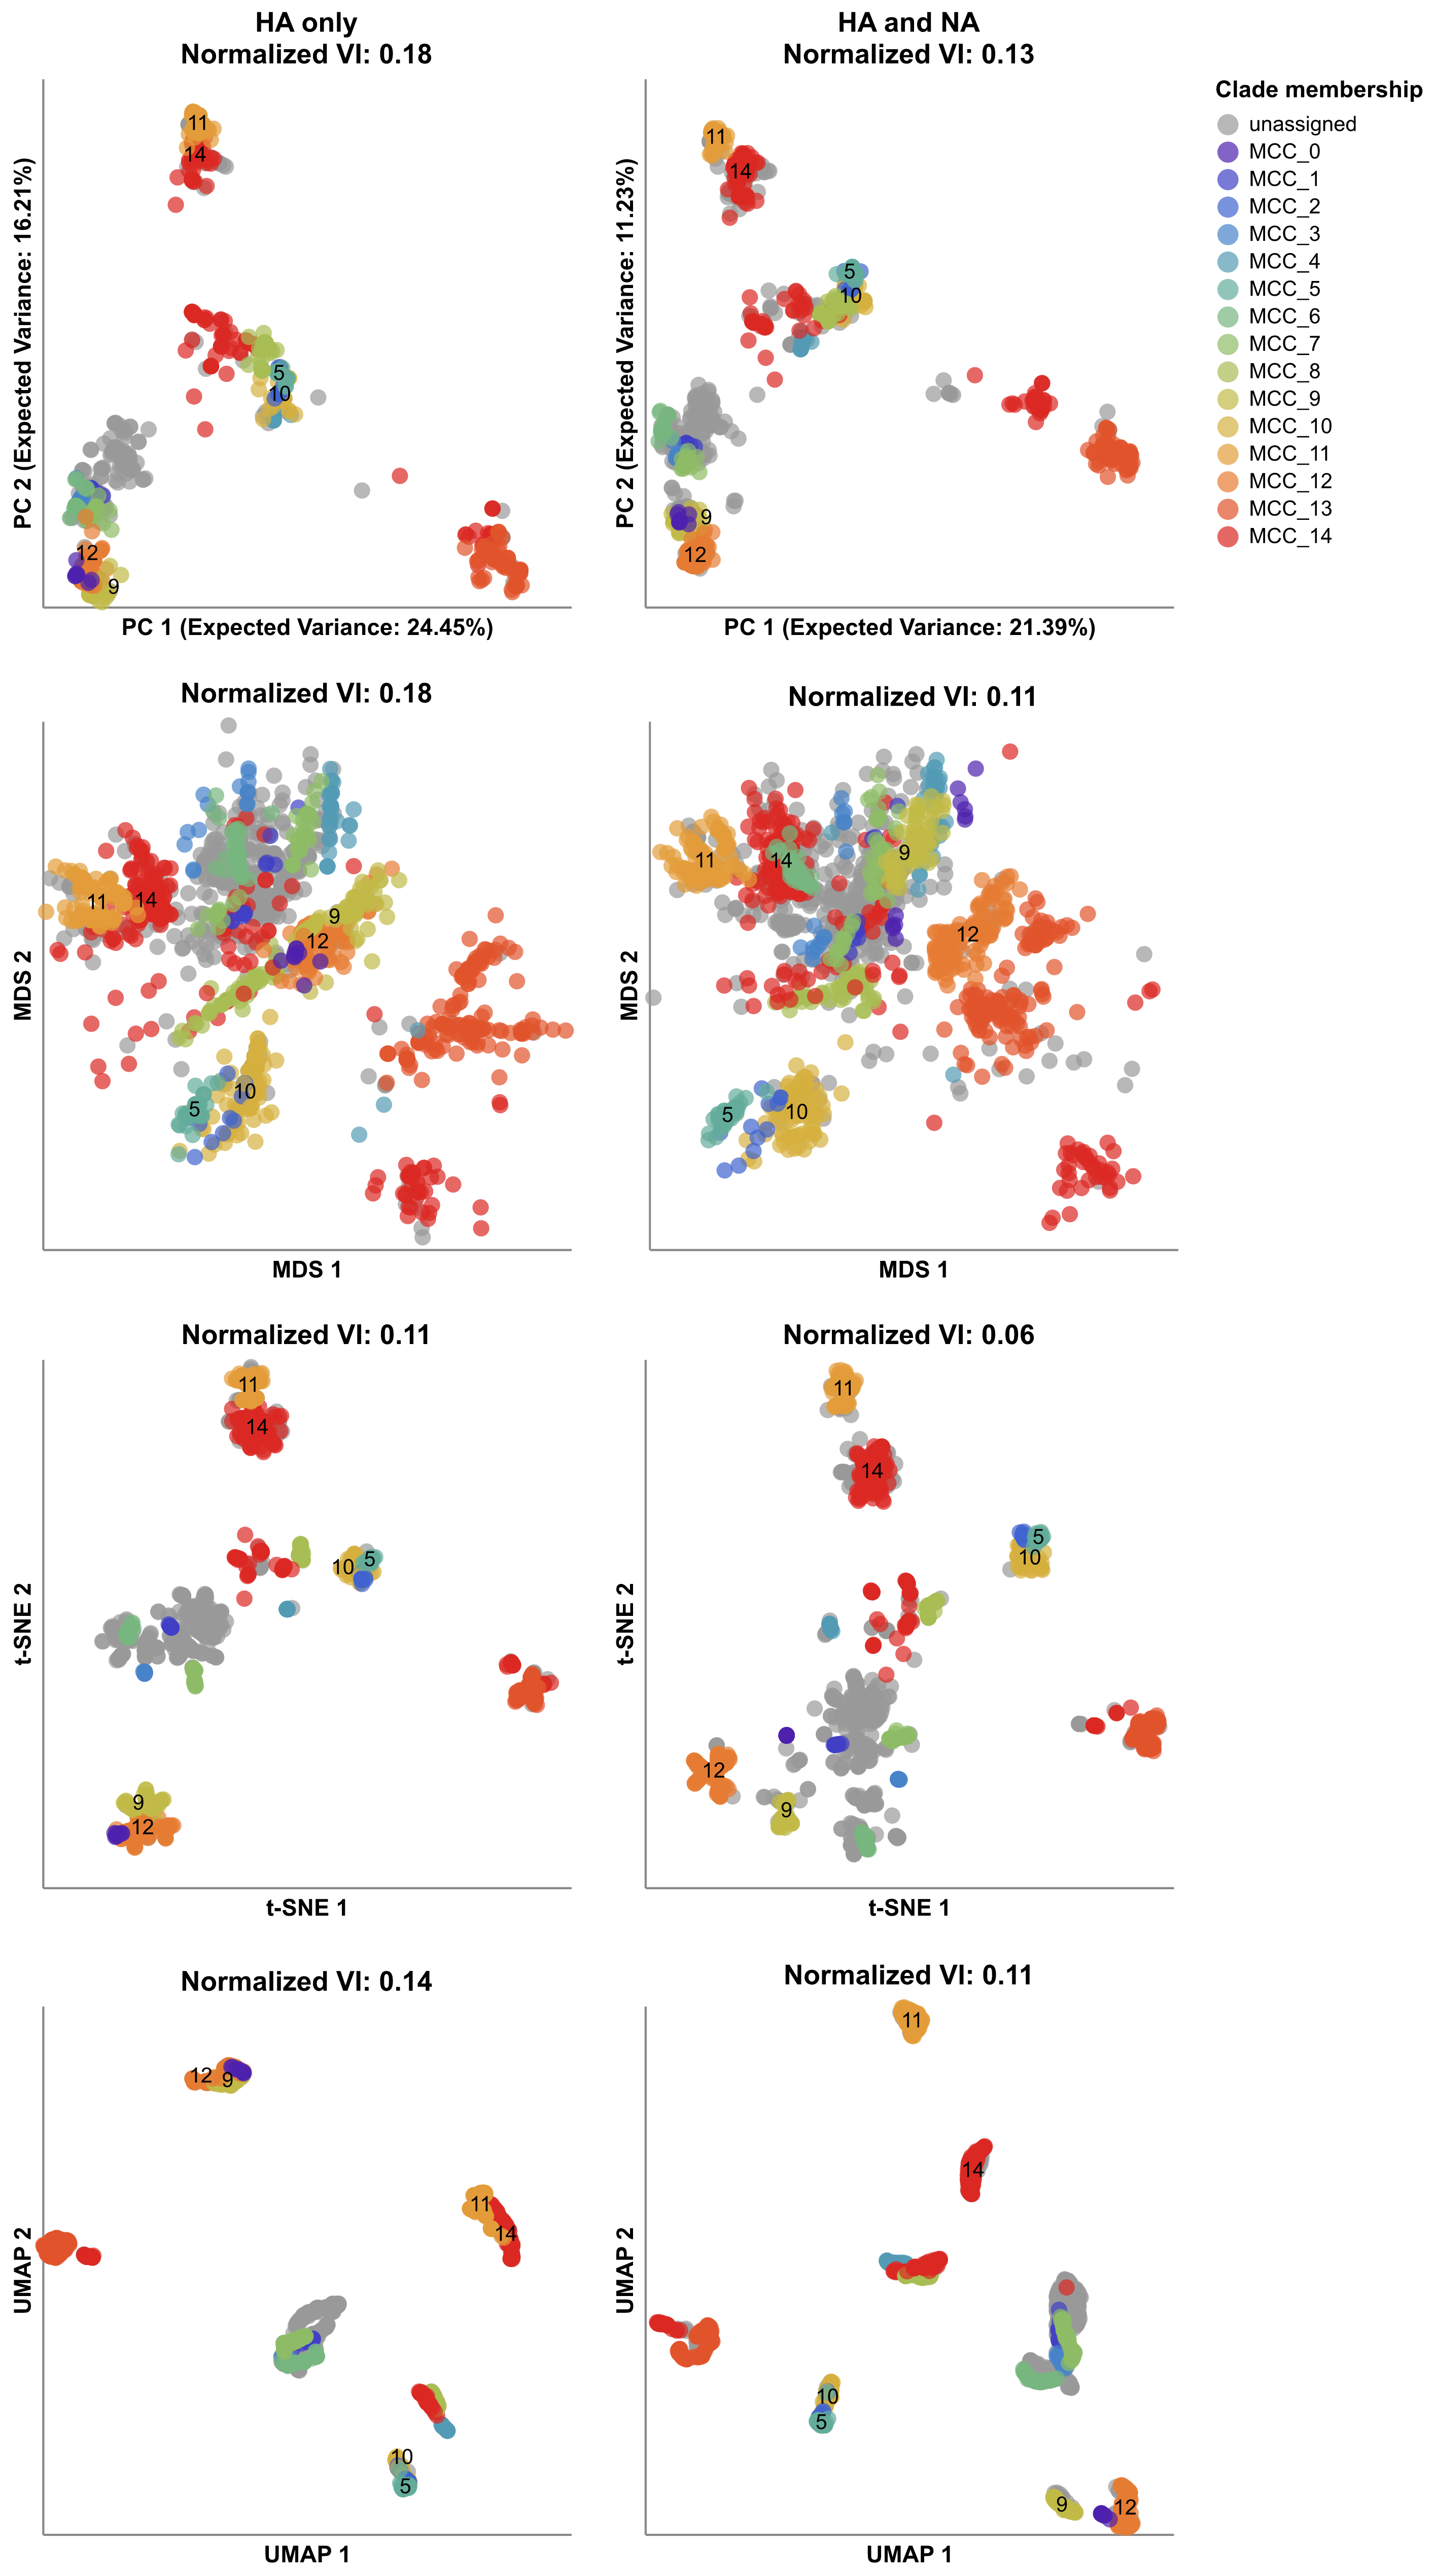
\includegraphics[width=0.75\columnwidth]{figures/flu-2016-2018-ha-na-all-embeddings-by-mcc.png}
\caption{{\bf Embeddings influenza H3N2 HA-only (left) and combined HA/NA (right) showing the effects of additional NA genetic information on the placement of reassortment events detected by TreeKnit (MCCs).}}\label{S_Fig_full_ha_na_embeddings}
\end{figure}

\begin{figure}[!h]
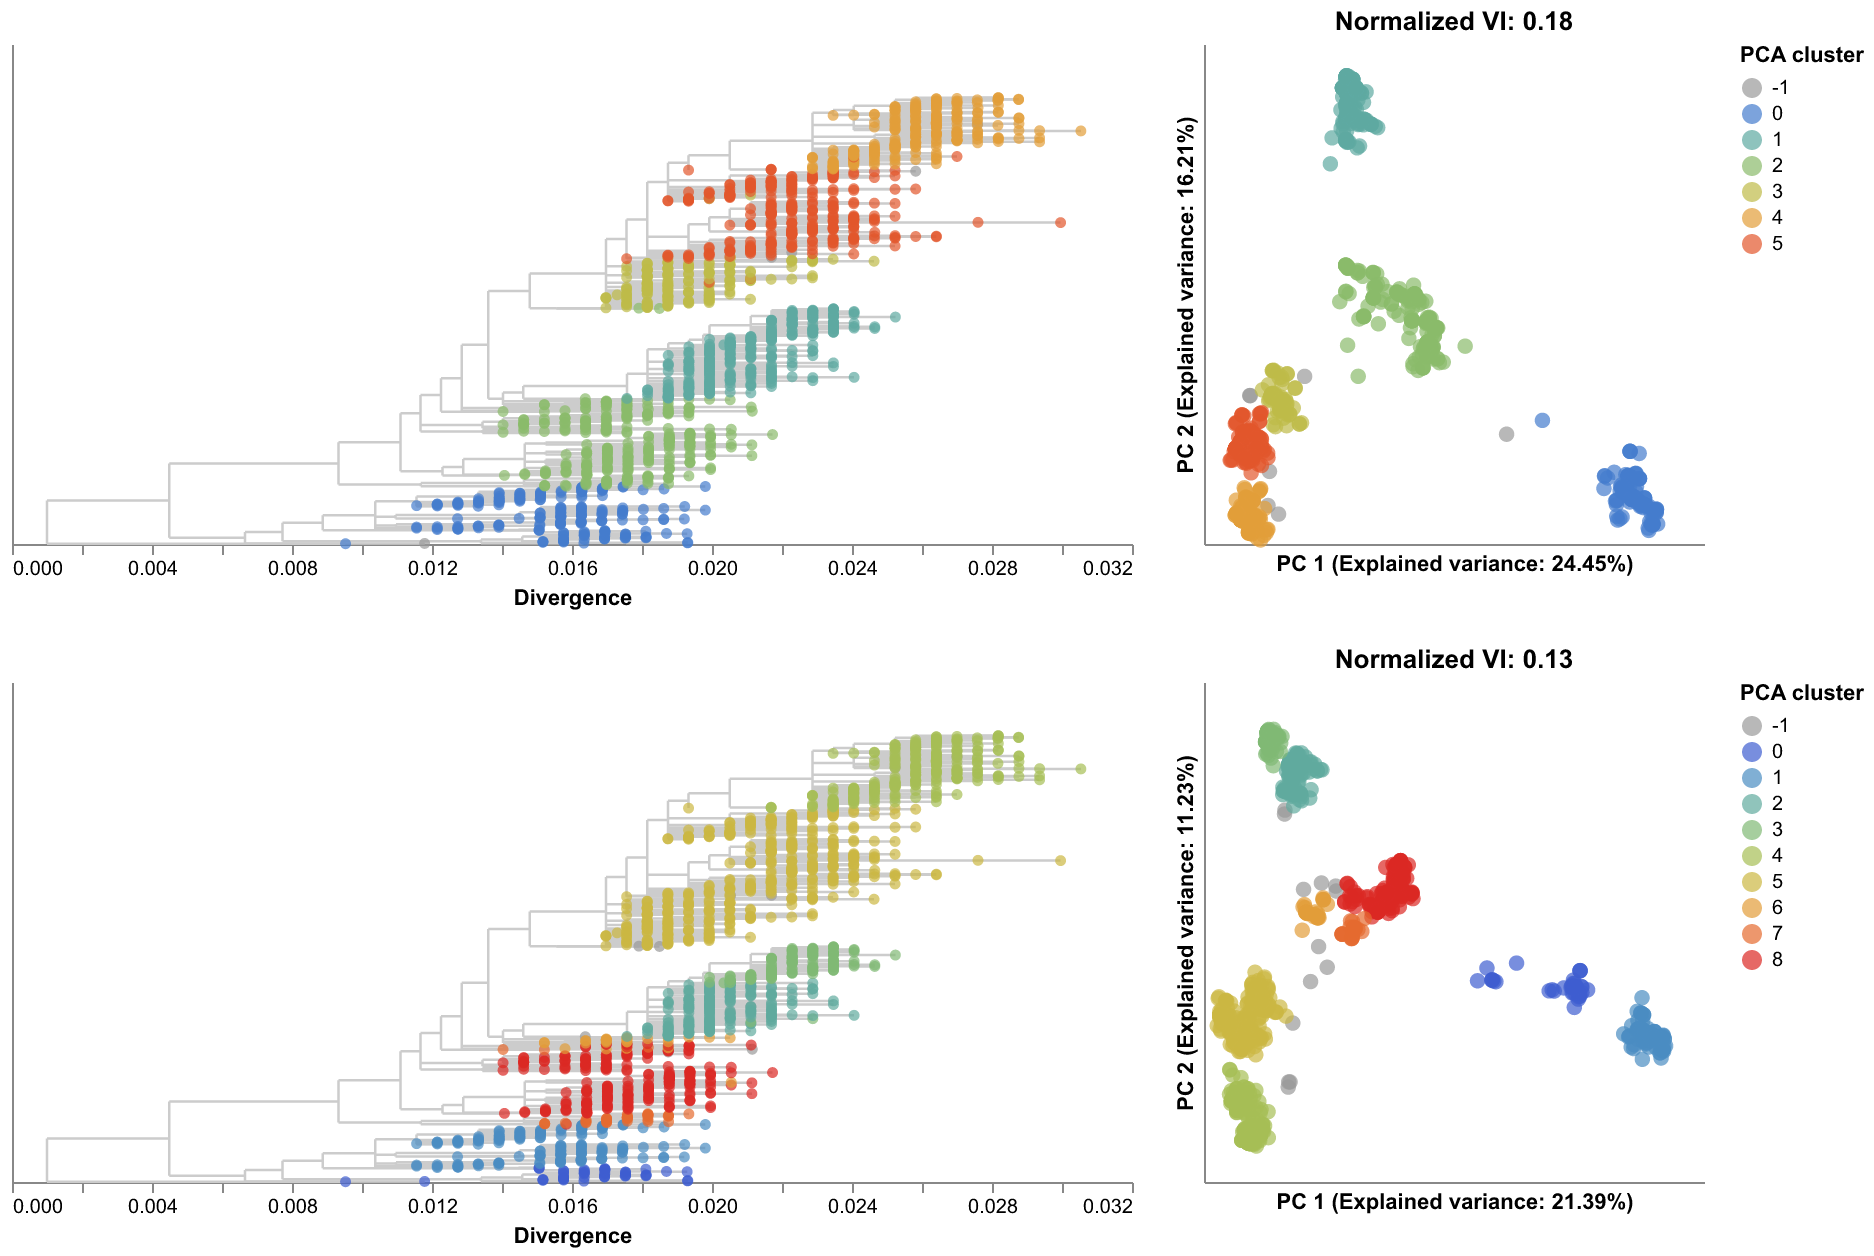
\includegraphics[width=\columnwidth]{figures/flu-2016-2018-ha-na-pca-by-cluster.png}
\caption{{\bf PCA embeddings for influenza H3N2 HA sequences only (top row) and HA/NA sequences combined (bottom row) showing the HA trees colored by clusters identified in each embedding (left) and the corresponding embeddings colored by cluster (right).}}\label{S_Fig_flu_ha_na_pca_embeddings}
\end{figure}

\begin{figure}[!h]
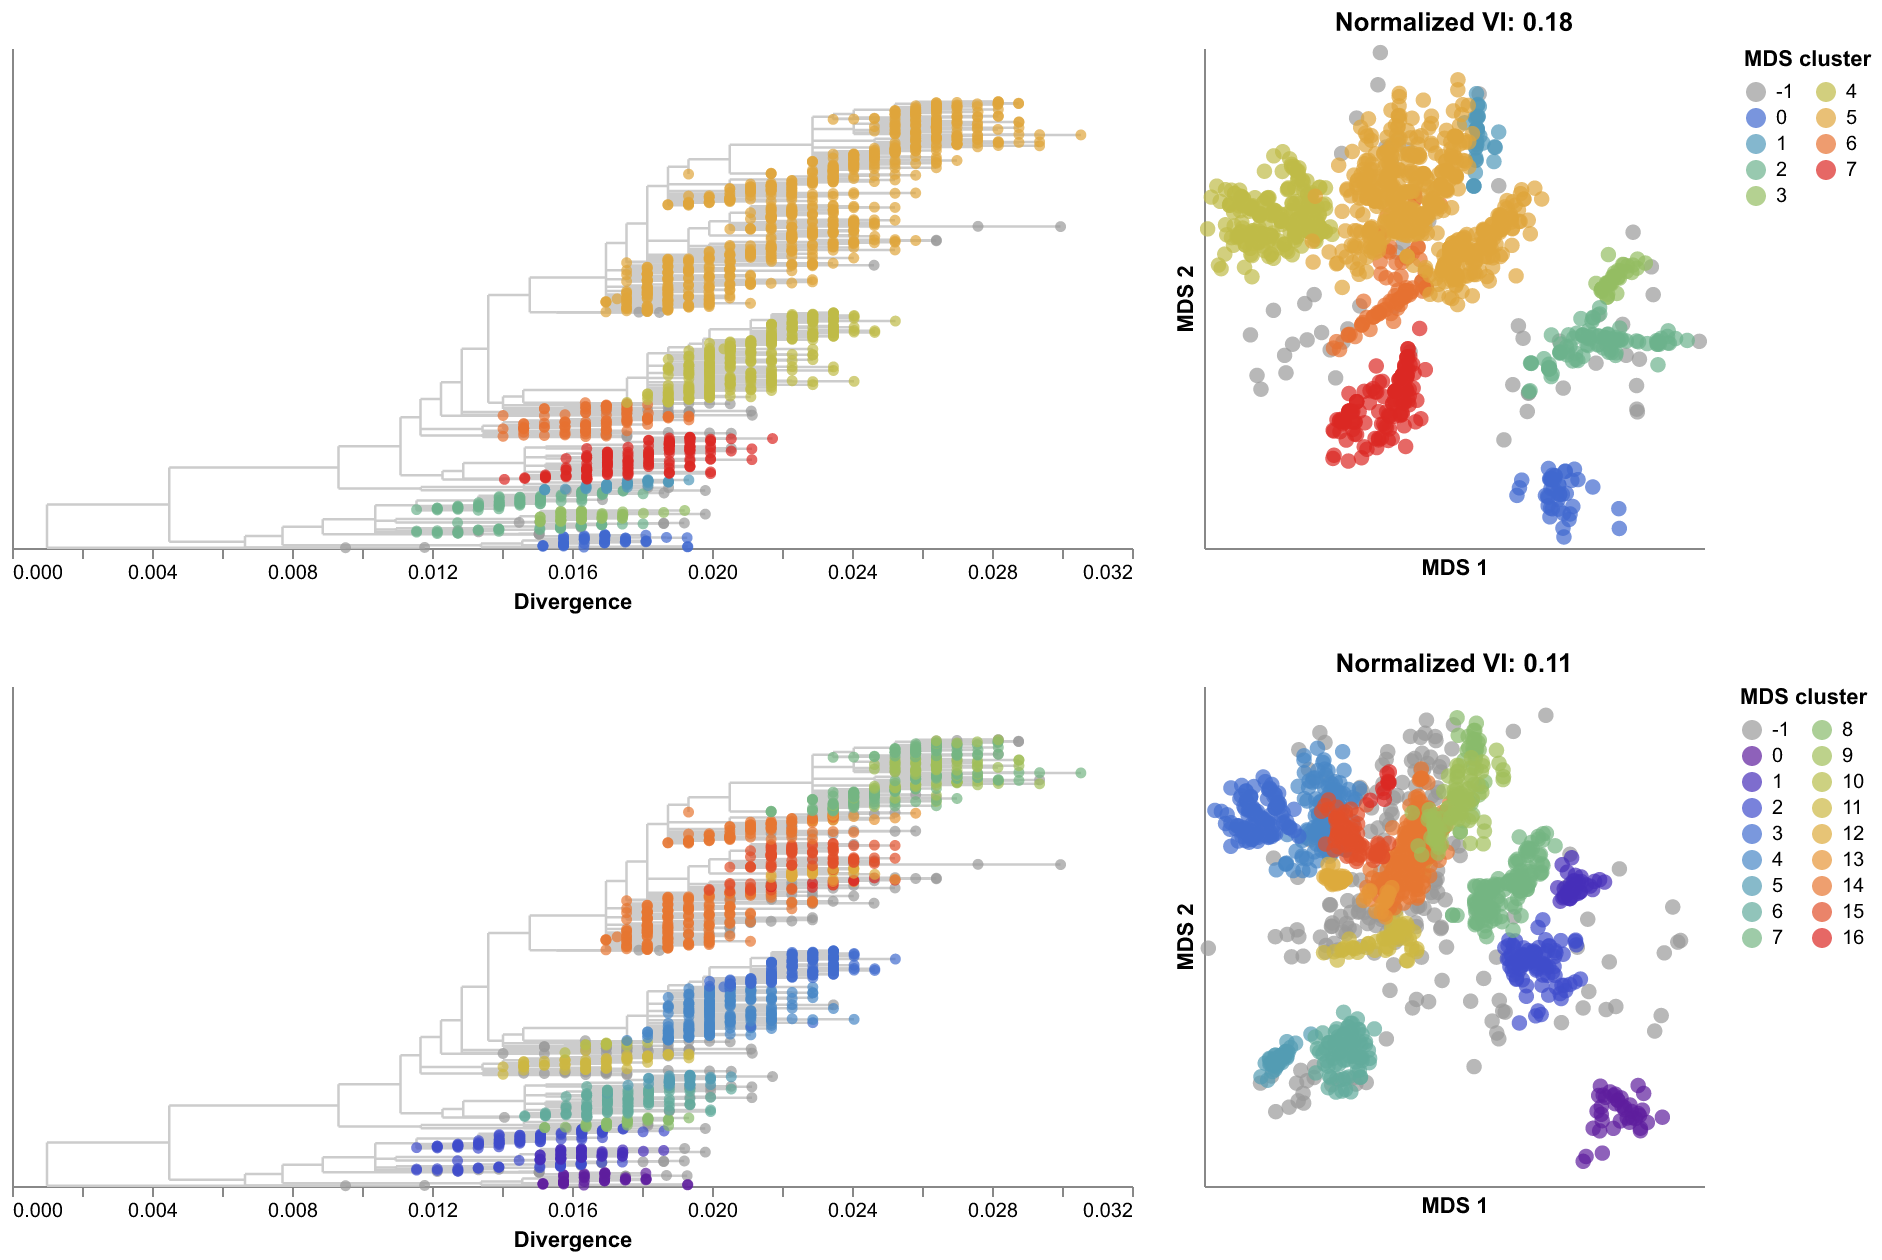
\includegraphics[width=\columnwidth]{figures/flu-2016-2018-ha-na-mds-by-cluster.png}
\caption{{\bf MDS embeddings for influenza H3N2 HA sequences only (top row) and HA/NA sequences combined (bottom row) showing the HA trees colored by clusters identified in each embedding (left) and the corresponding embeddings colored by cluster (right).}}\label{S_Fig_flu_ha_na_mds_embeddings}
\end{figure}

\begin{figure}[!h]
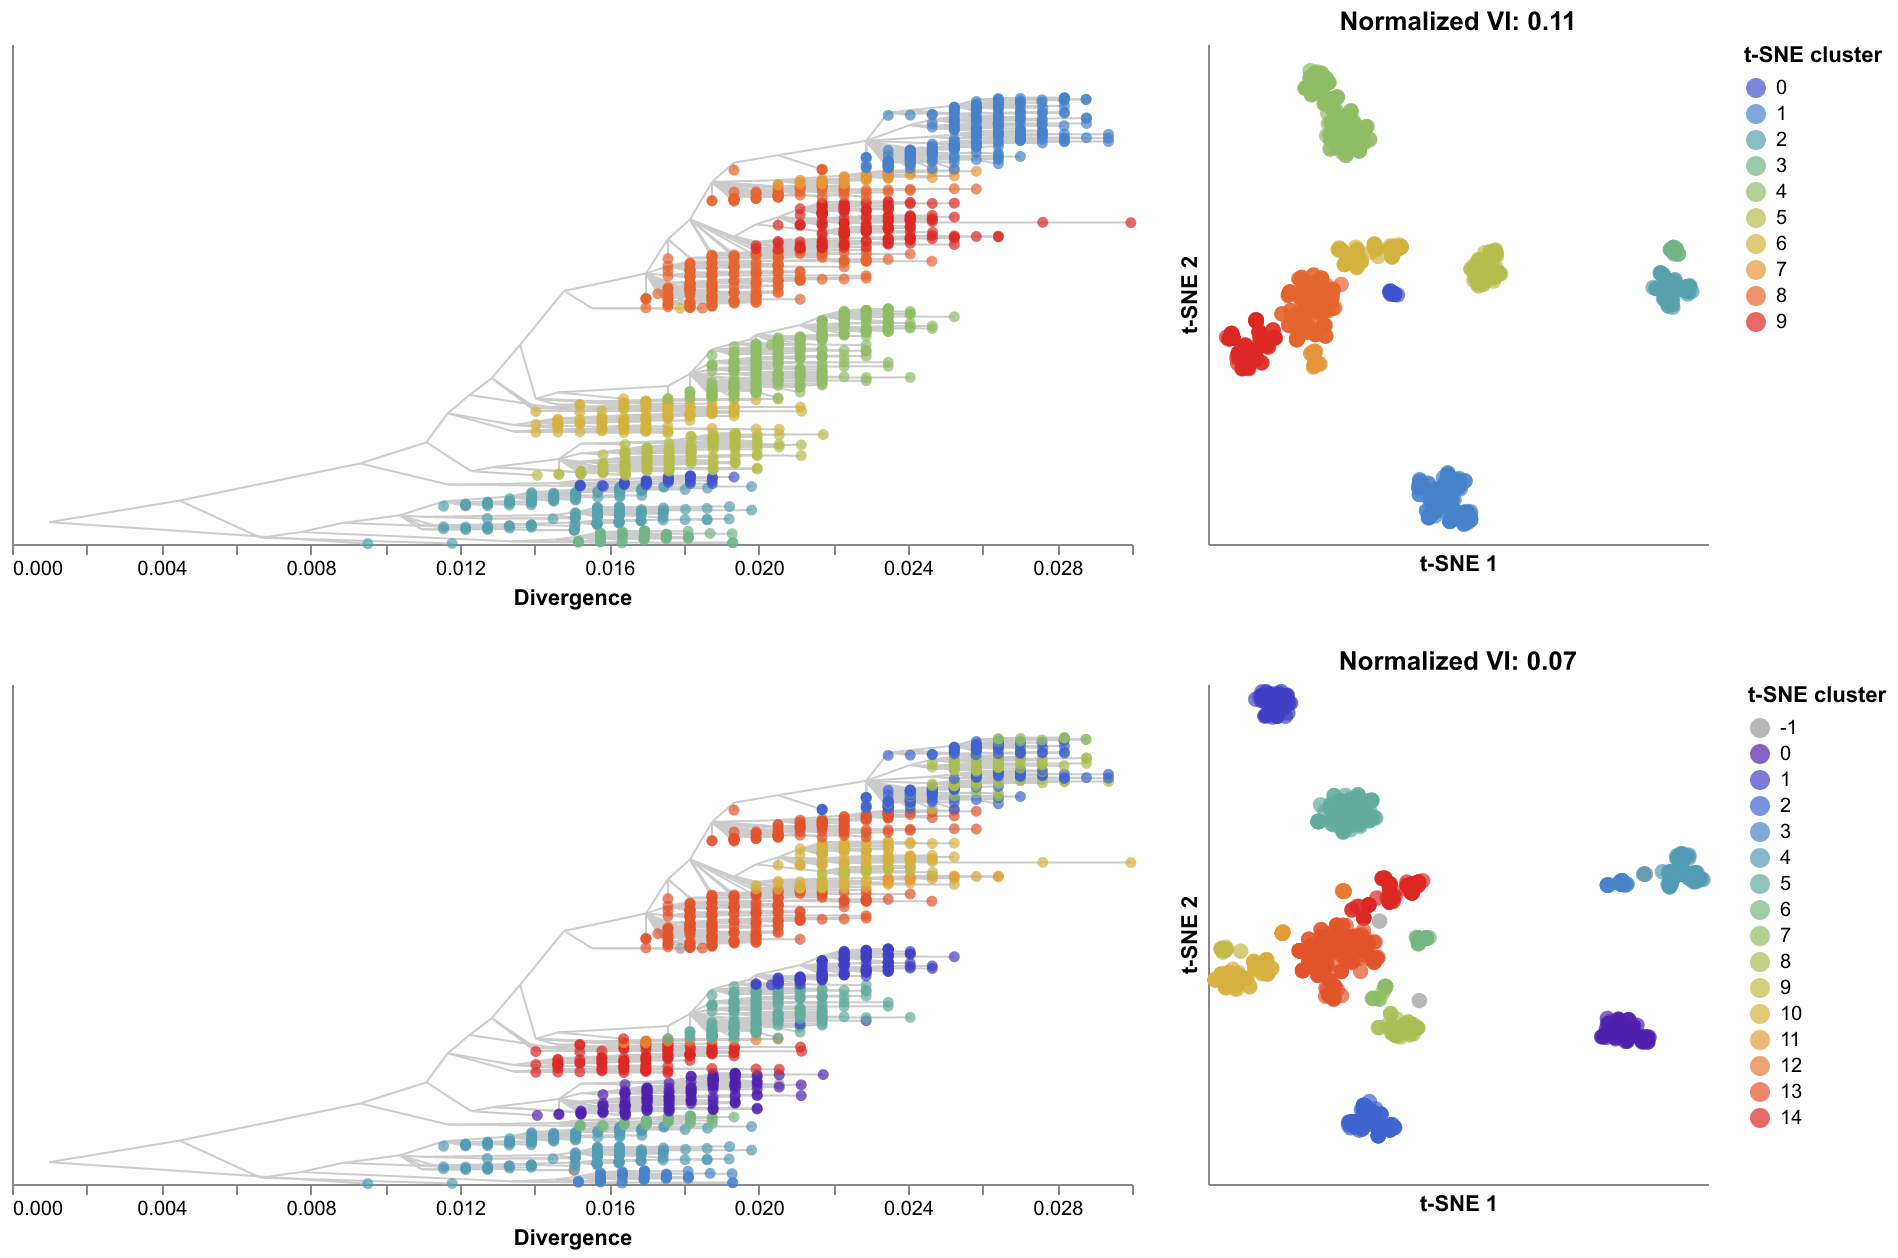
\includegraphics[width=\columnwidth]{figures/flu-2016-2018-ha-na-tsne-by-cluster.png}
\caption{{\bf t-SNE embeddings for influenza H3N2 HA sequences only (top row) and HA/NA sequences combined (bottom row) showing the HA trees colored by clusters identified in each embedding (left) and the corresponding embeddings colored by cluster (right).}}\label{S_Fig_flu_ha_na_tsne_embeddings}
\end{figure}

\begin{figure}[!h]
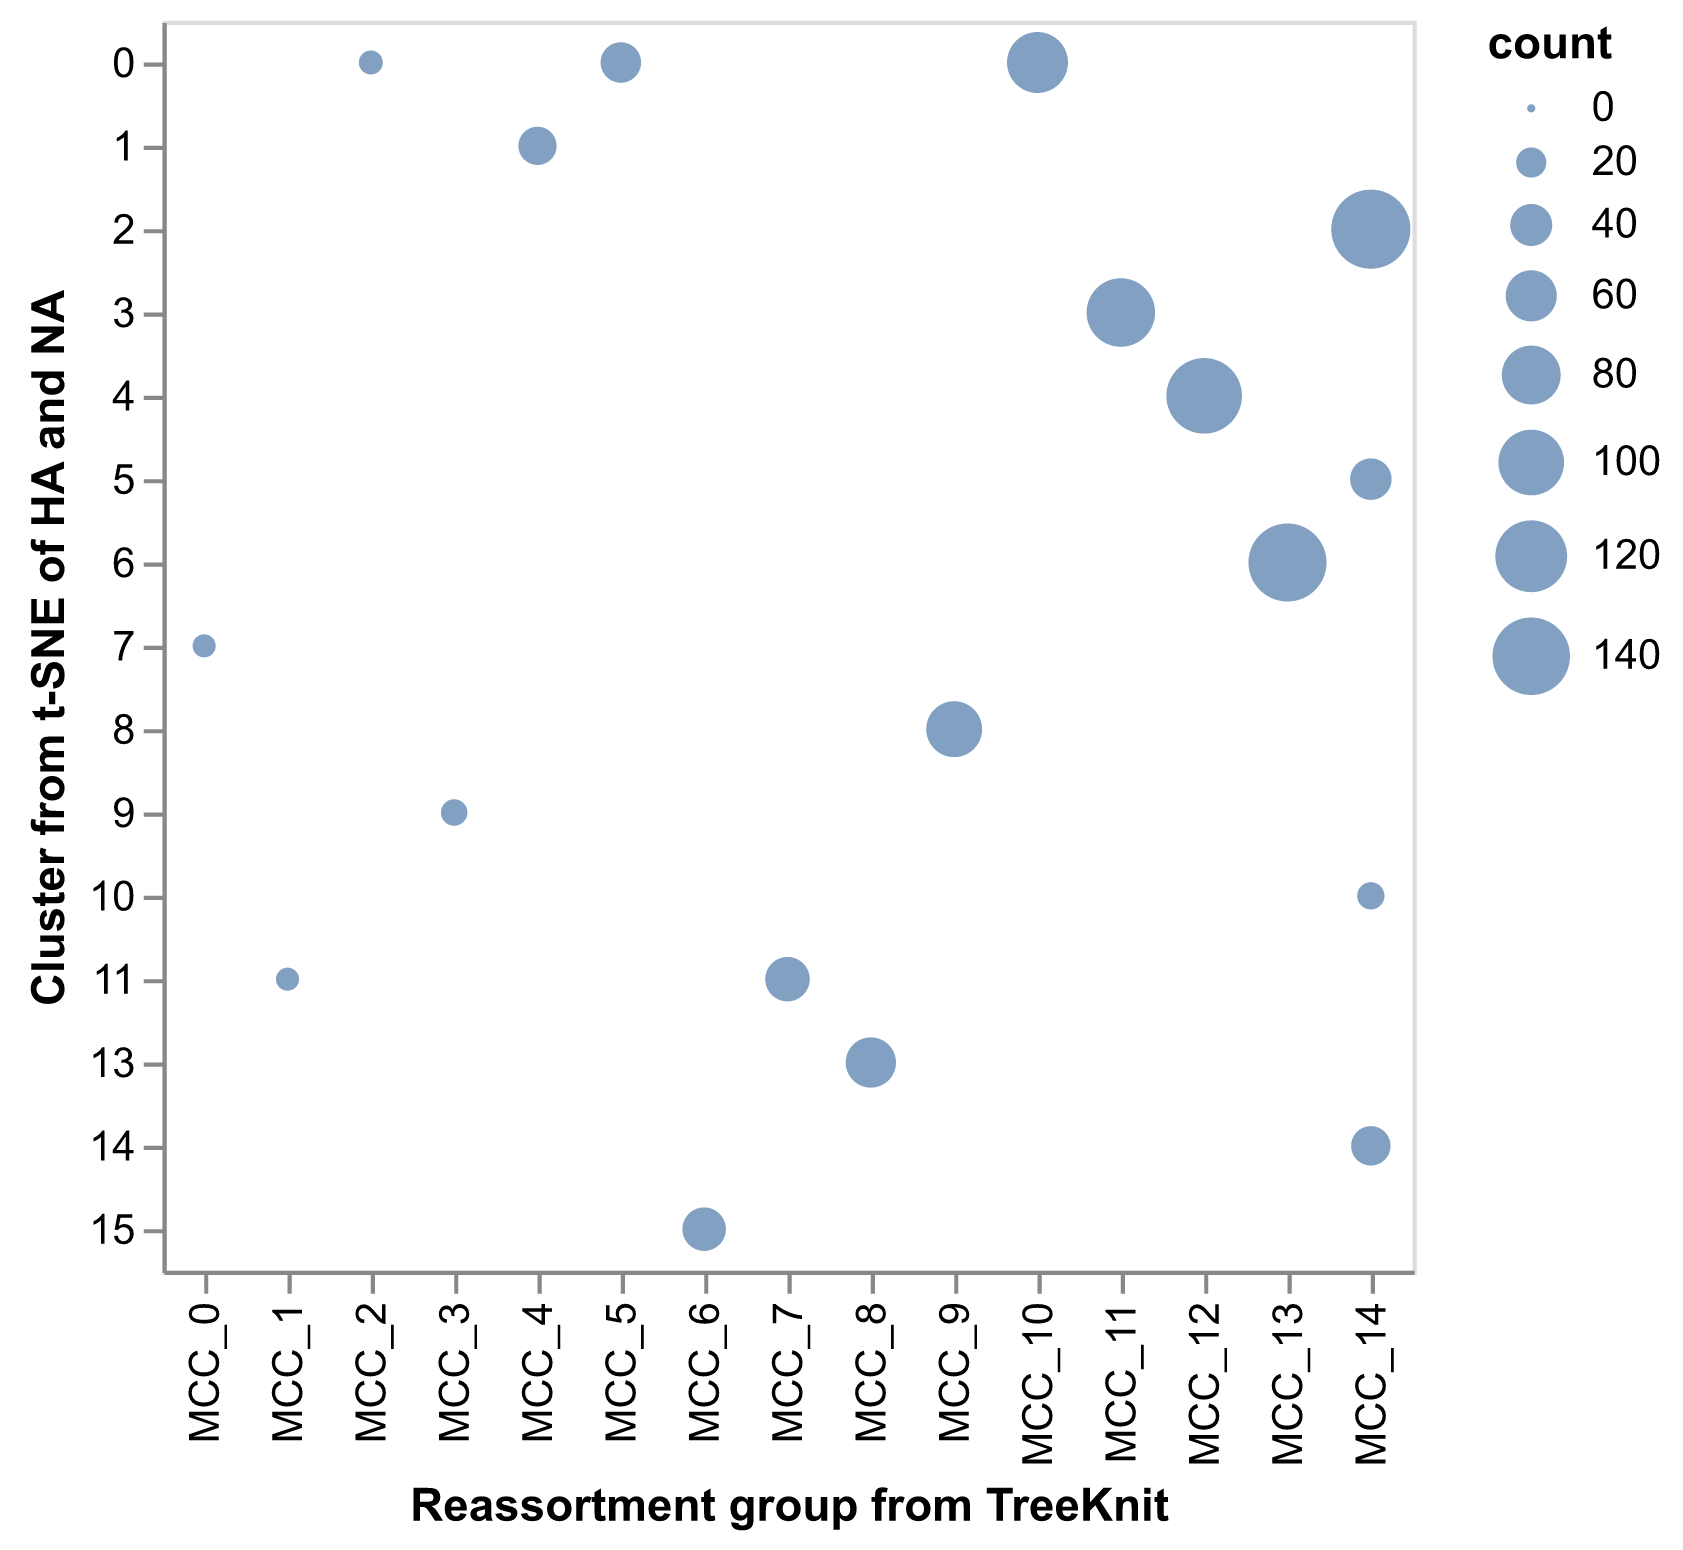
\includegraphics[width=\columnwidth]{figures/flu-2016-2018-ha-na-tsne-mcc-counts.png}
\caption{{\bf Number of H3N2 strains per combination of reassortment group identified with TreeKnit (MCCs) and cluster identified from joint t-SNE embeddings of HA and NA where the count was at least 10 strains.}}\label{S_Fig_flu_ha_na_tsne_mcc_counts}
\end{figure}

\begin{figure}[!h]
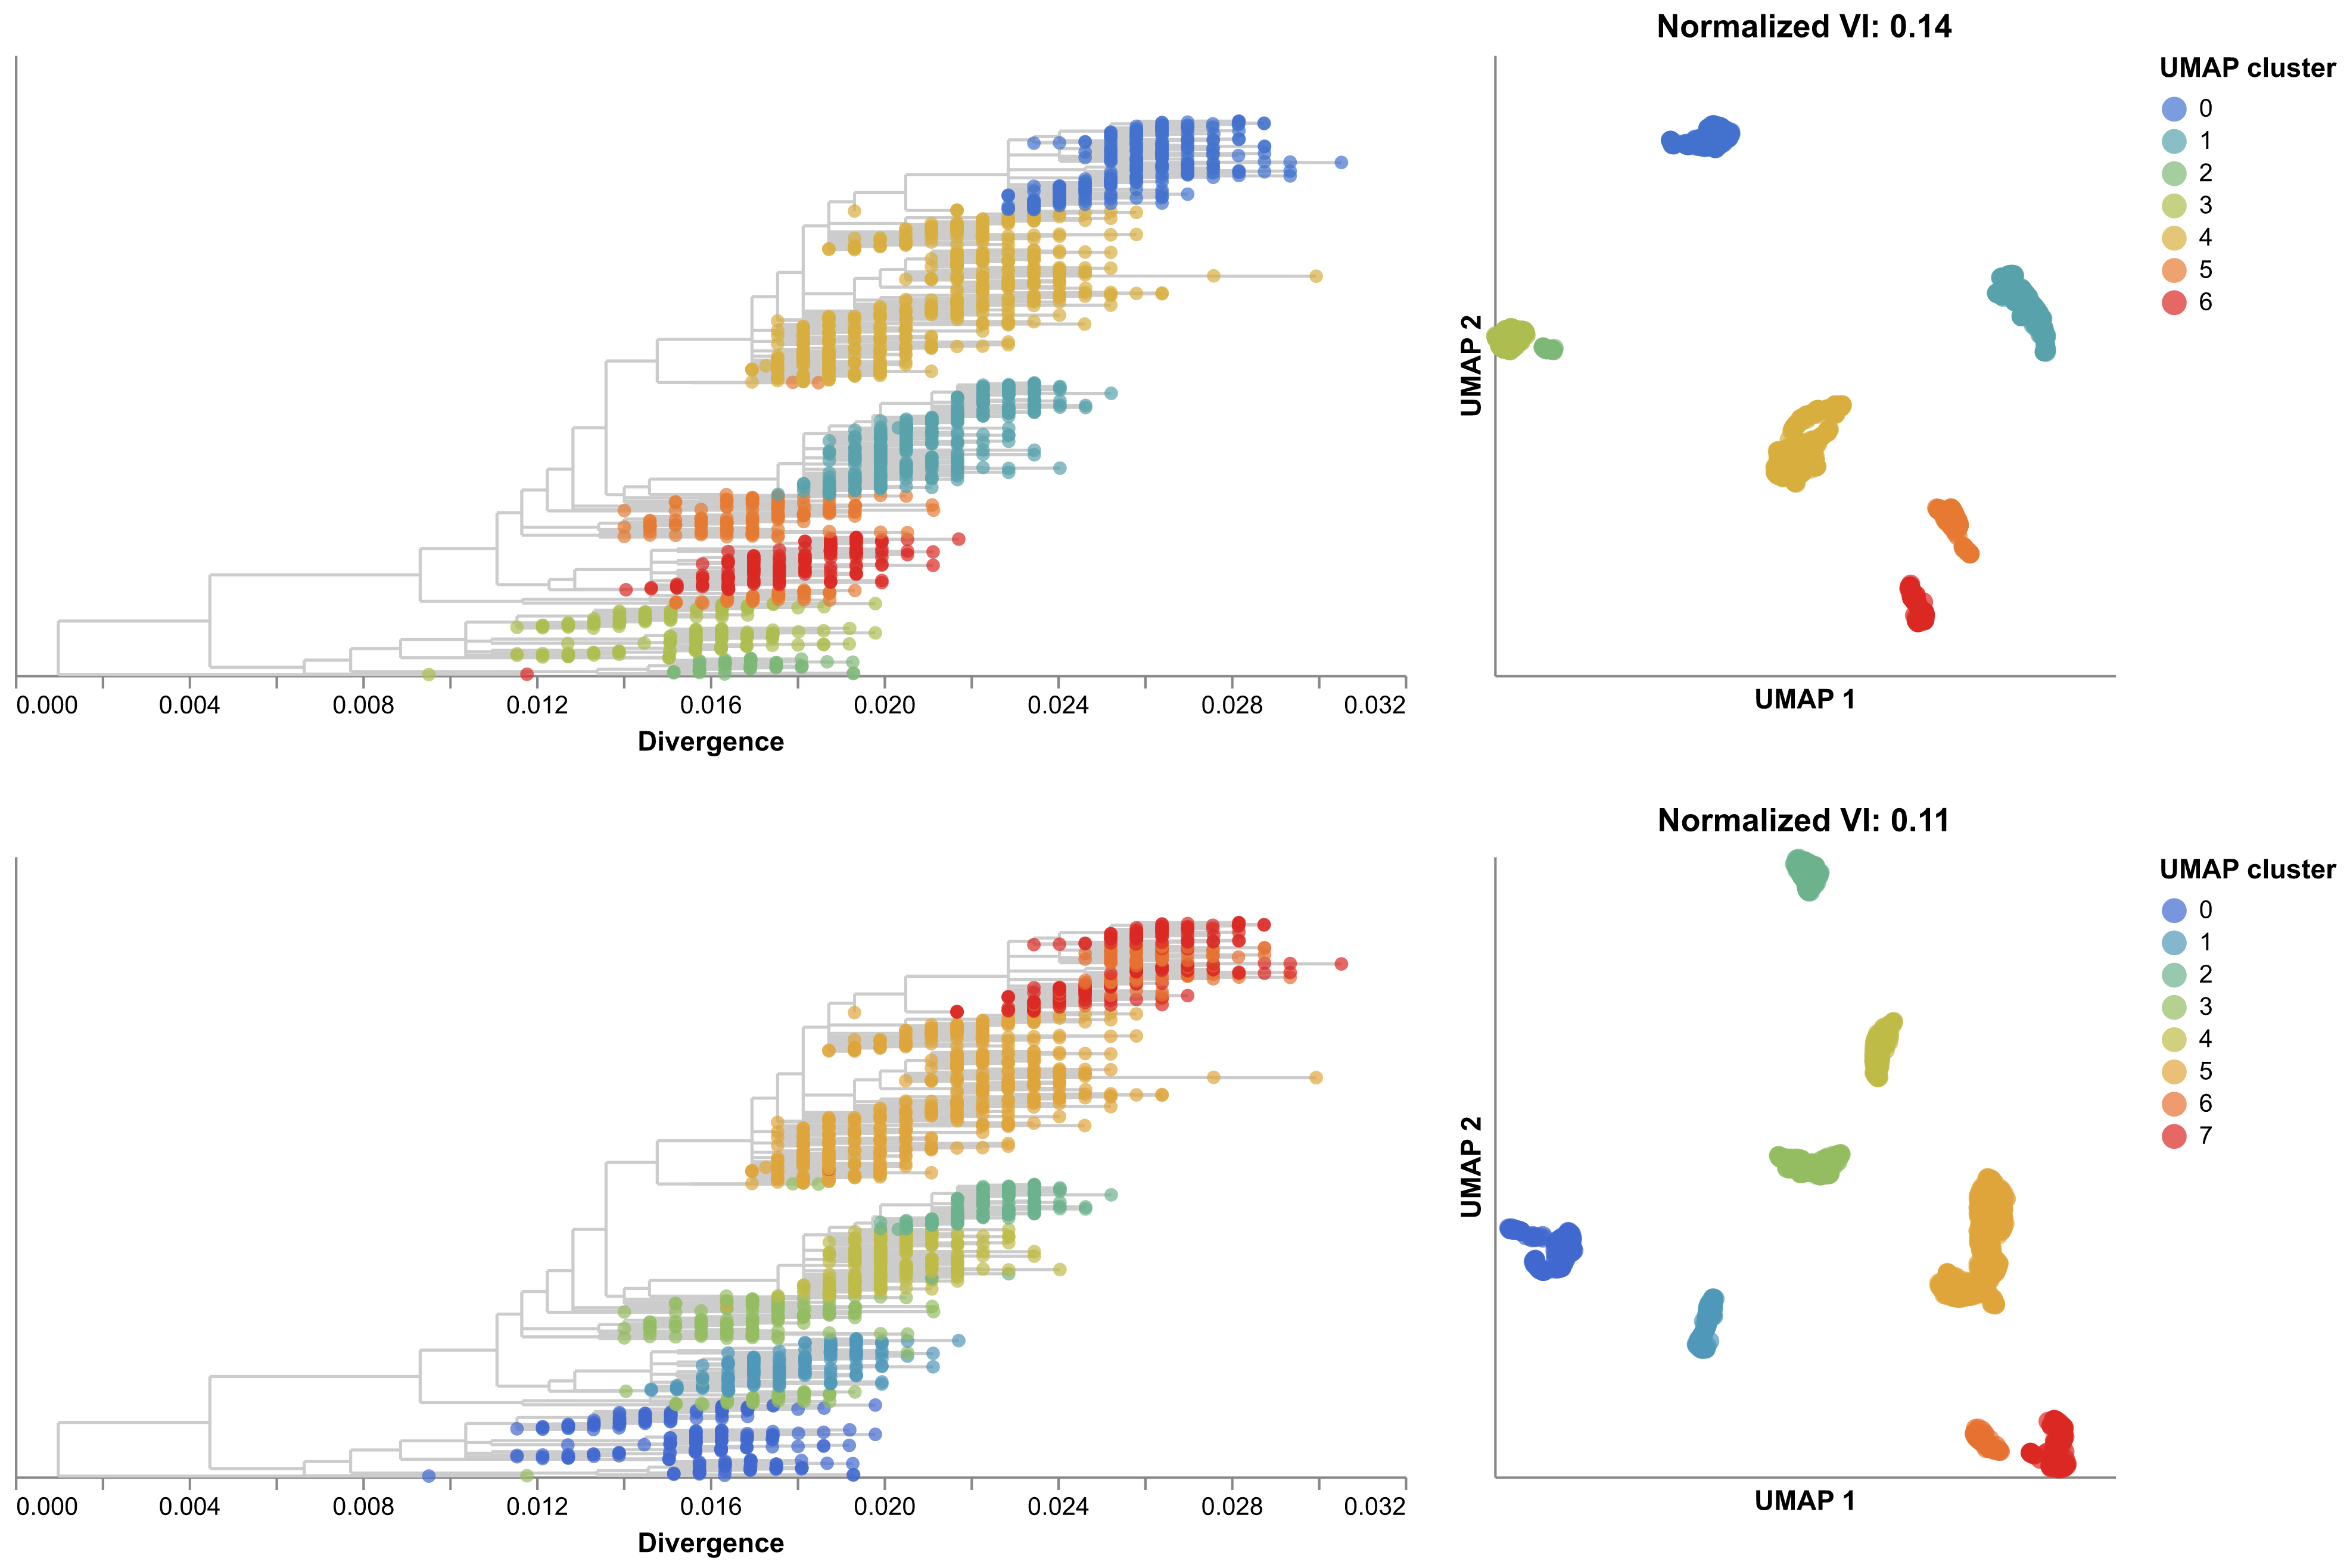
\includegraphics[width=\columnwidth]{figures/flu-2016-2018-ha-na-umap-by-cluster.png}
\caption{{\bf UMAP embeddings for influenza H3N2 HA sequences only (top row) and HA/NA sequences combined (bottom row) showing the HA trees colored by clusters identified in each embedding (left) and the corresponding embeddings colored by cluster (right).}}\label{S_Fig_flu_ha_na_umap_embeddings}
\end{figure}

\begin{figure}[!h]
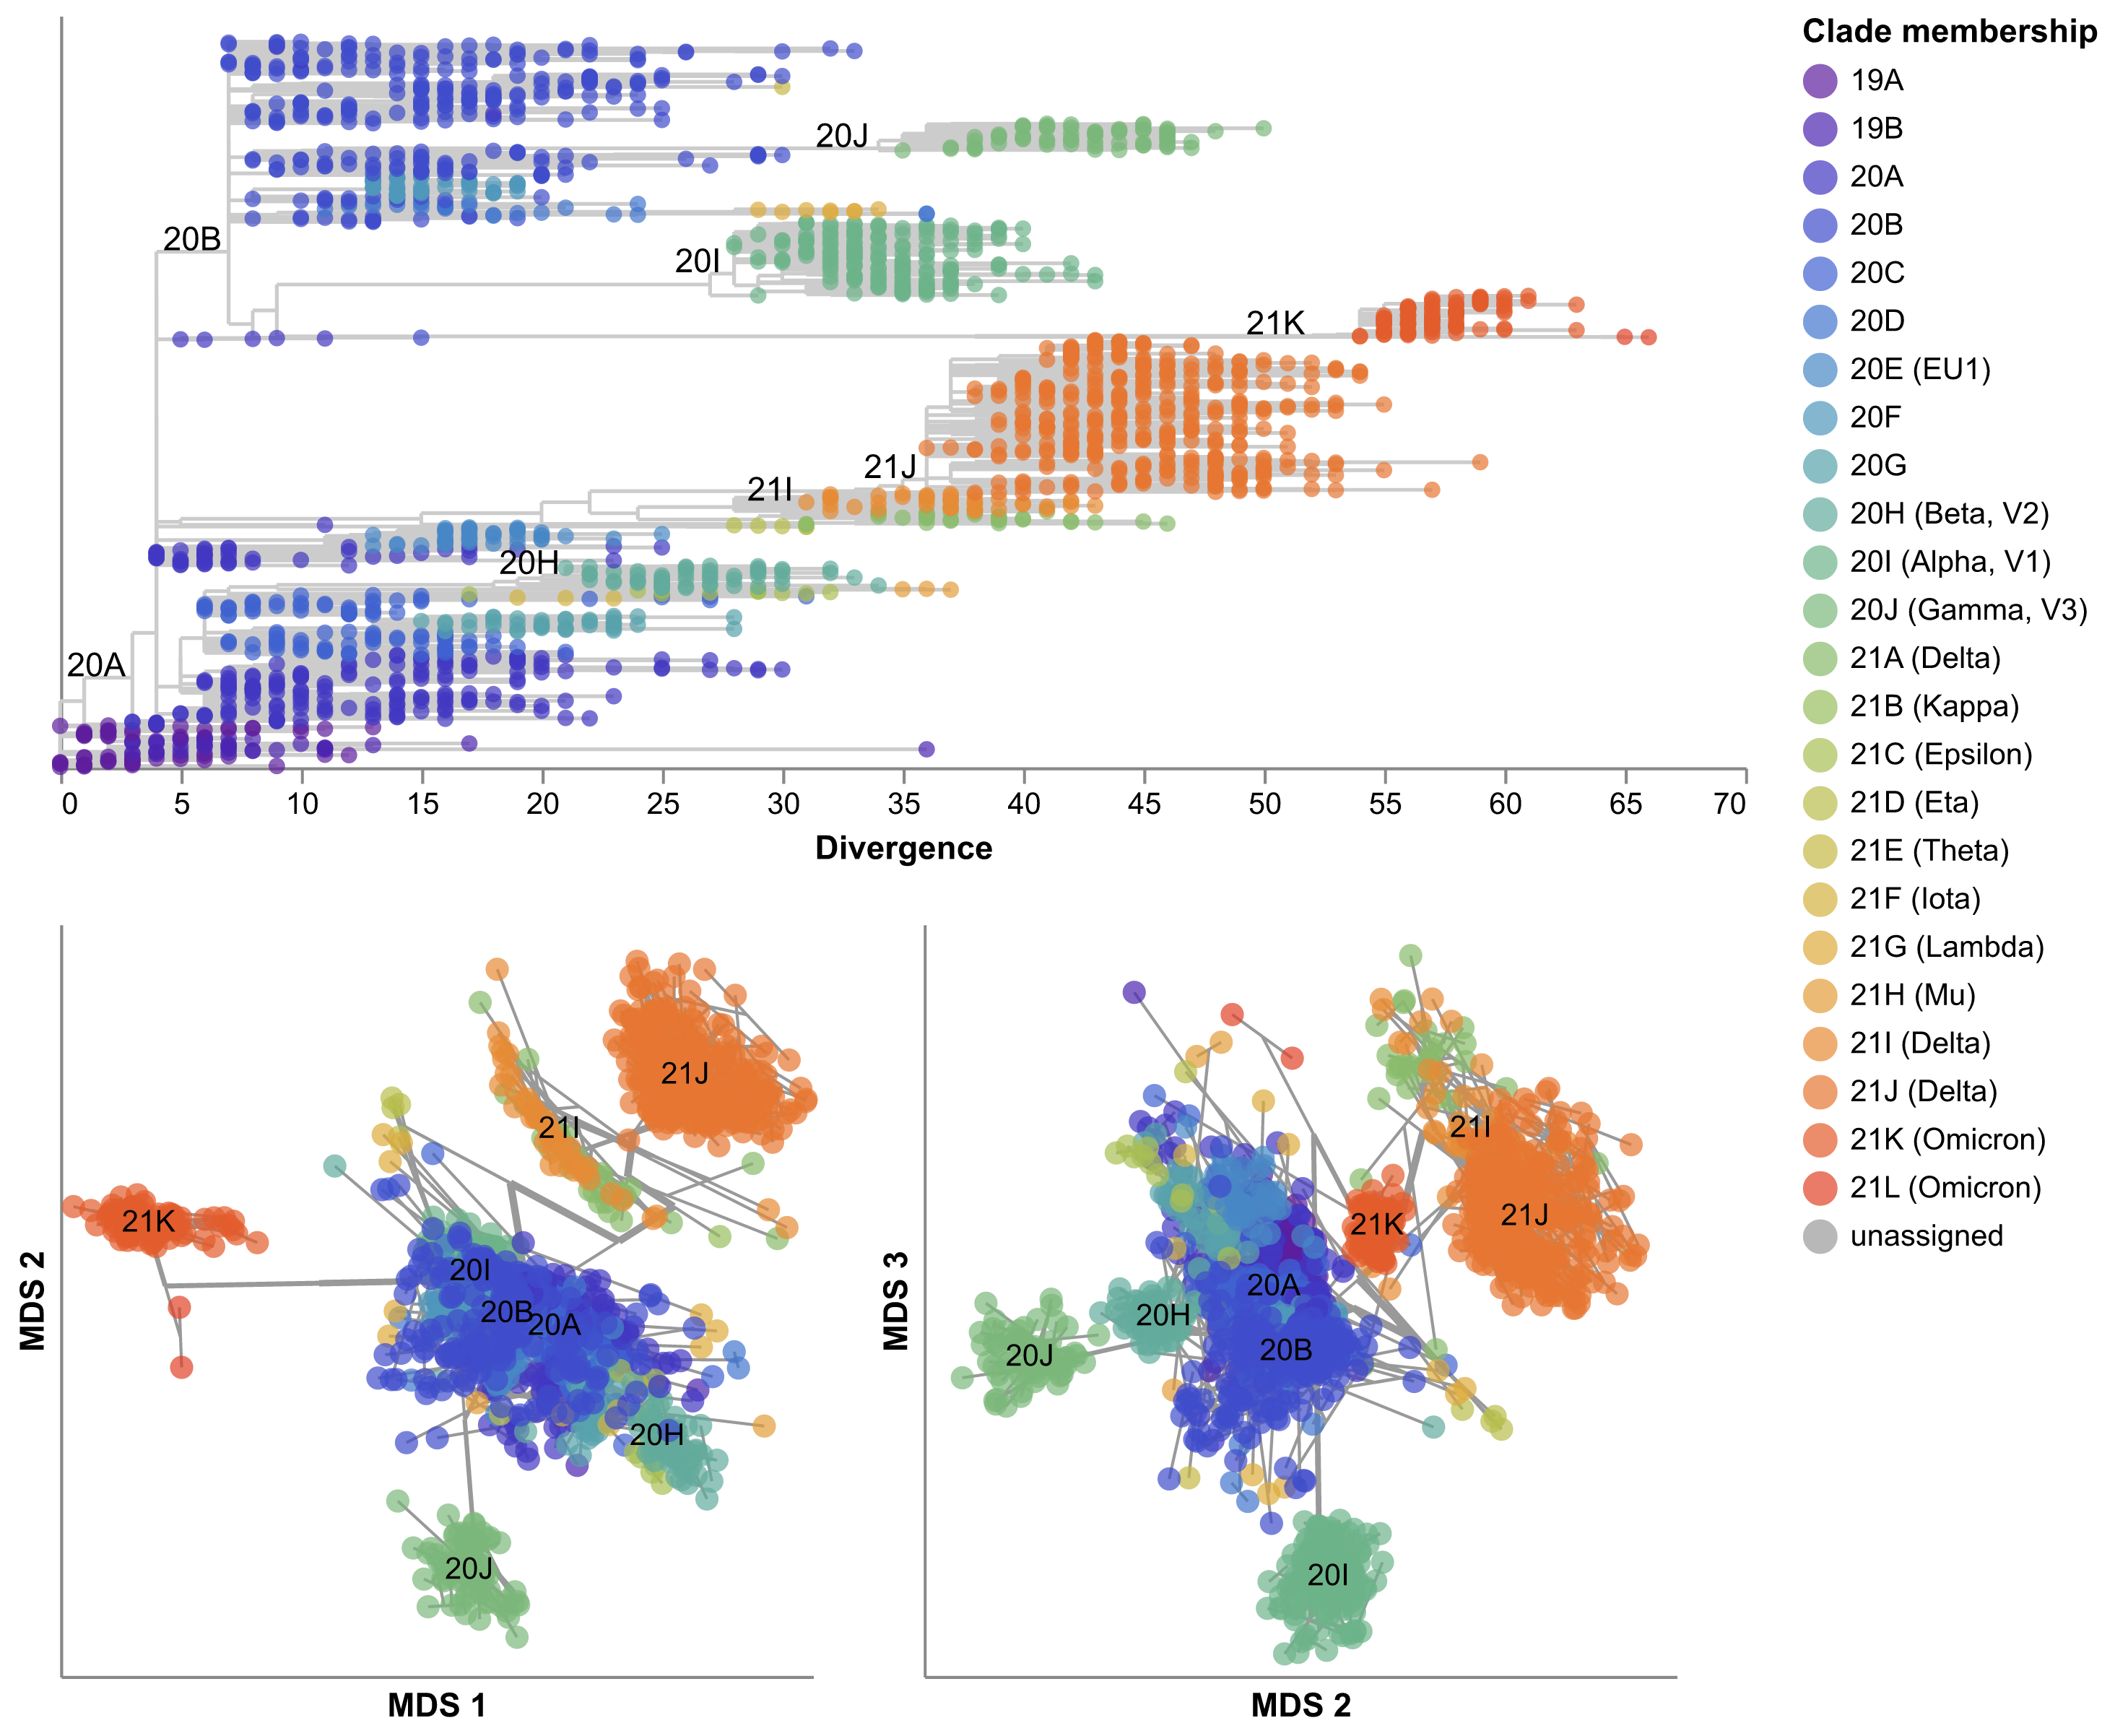
\includegraphics[width=\columnwidth]{figures/sarscov2-mds-by-Nextstrain_clade-clade.png}
\caption{{\bf MDS embeddings for early SARS-CoV-2 sequences showing all three components.}
  Line segments in each embedding reflect phylogenetic relationships with internal node positions calculated from the mean positions of their immediate descendants in each dimension (see Methods).
  Line thickness scales by the square root of the number of leaves descending from a given node in the phylogeny.}\label{S_Fig_sarscov2_early_mds}
\end{figure}

\begin{figure}[!h]
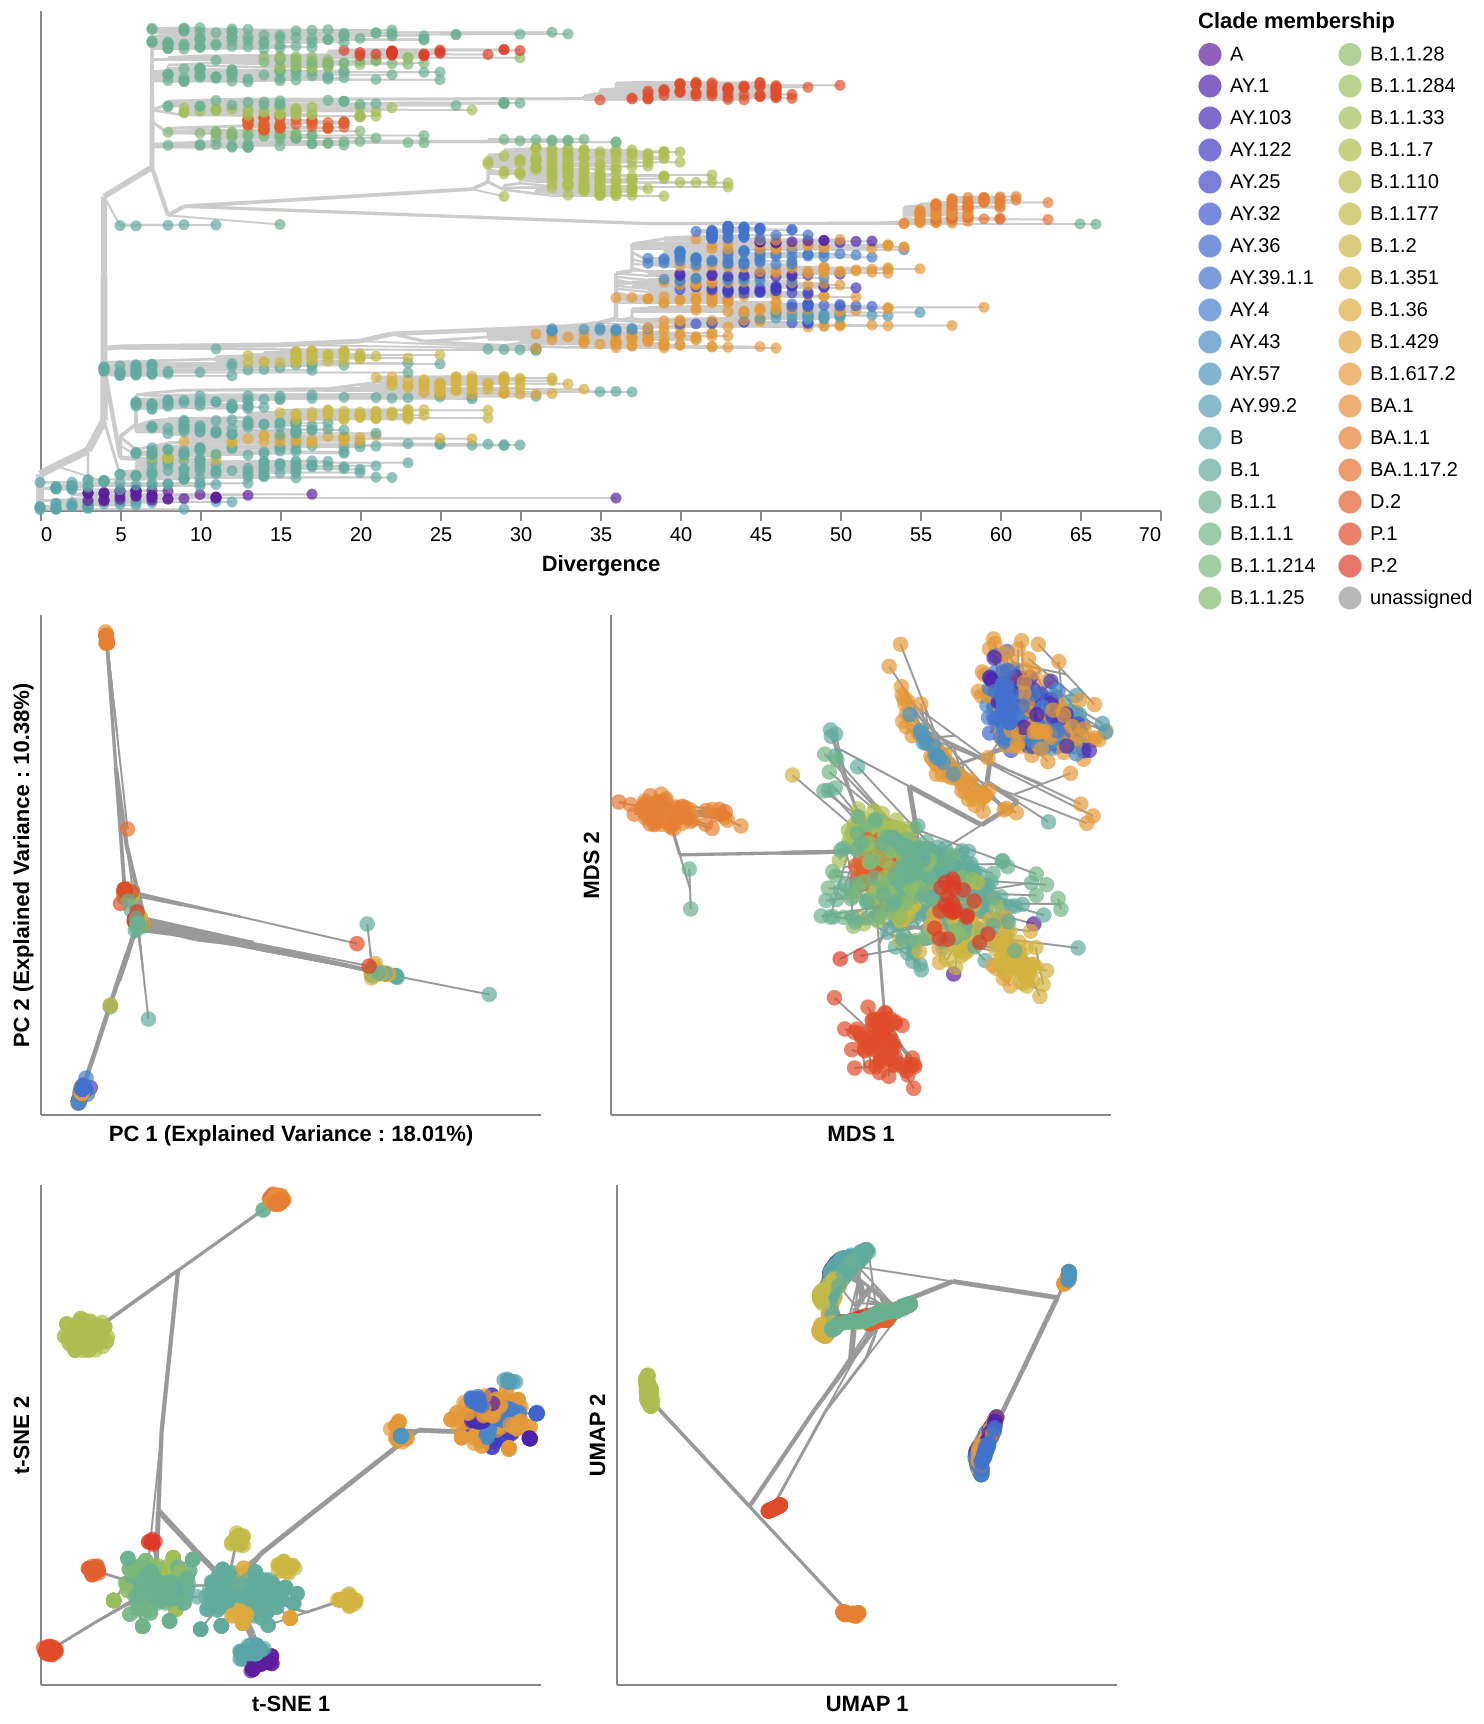
\includegraphics[width=\columnwidth]{figures/sarscov2-embeddings-by-Nextclade_pango_collapsed-clade.png}
\caption{{\bf Phylogeny of early (2020--2022) SARS-CoV-2 sequences plotted by number of nucleotide substitutions from the most recent common ancestor on the x-axis (top) and low-dimensional embeddings of the same sequences by PCA (middle left), MDS (middle right), t-SNE (bottom left), and UMAP (bottom right).}
  Tips in the tree and embeddings are colored by their Pango lineage assignment.
  Line segments in each embedding reflect phylogenetic relationships with internal node positions calculated from the mean positions of their immediate descendants in each dimension (see Methods).
  Line thickness scales by the square root of the number of leaves descending from a given node in the phylogeny.
}\label{S_Fig_sarscov2_early_embeddings_by_Nextclade_pango}
\end{figure}

\begin{figure}[!h]
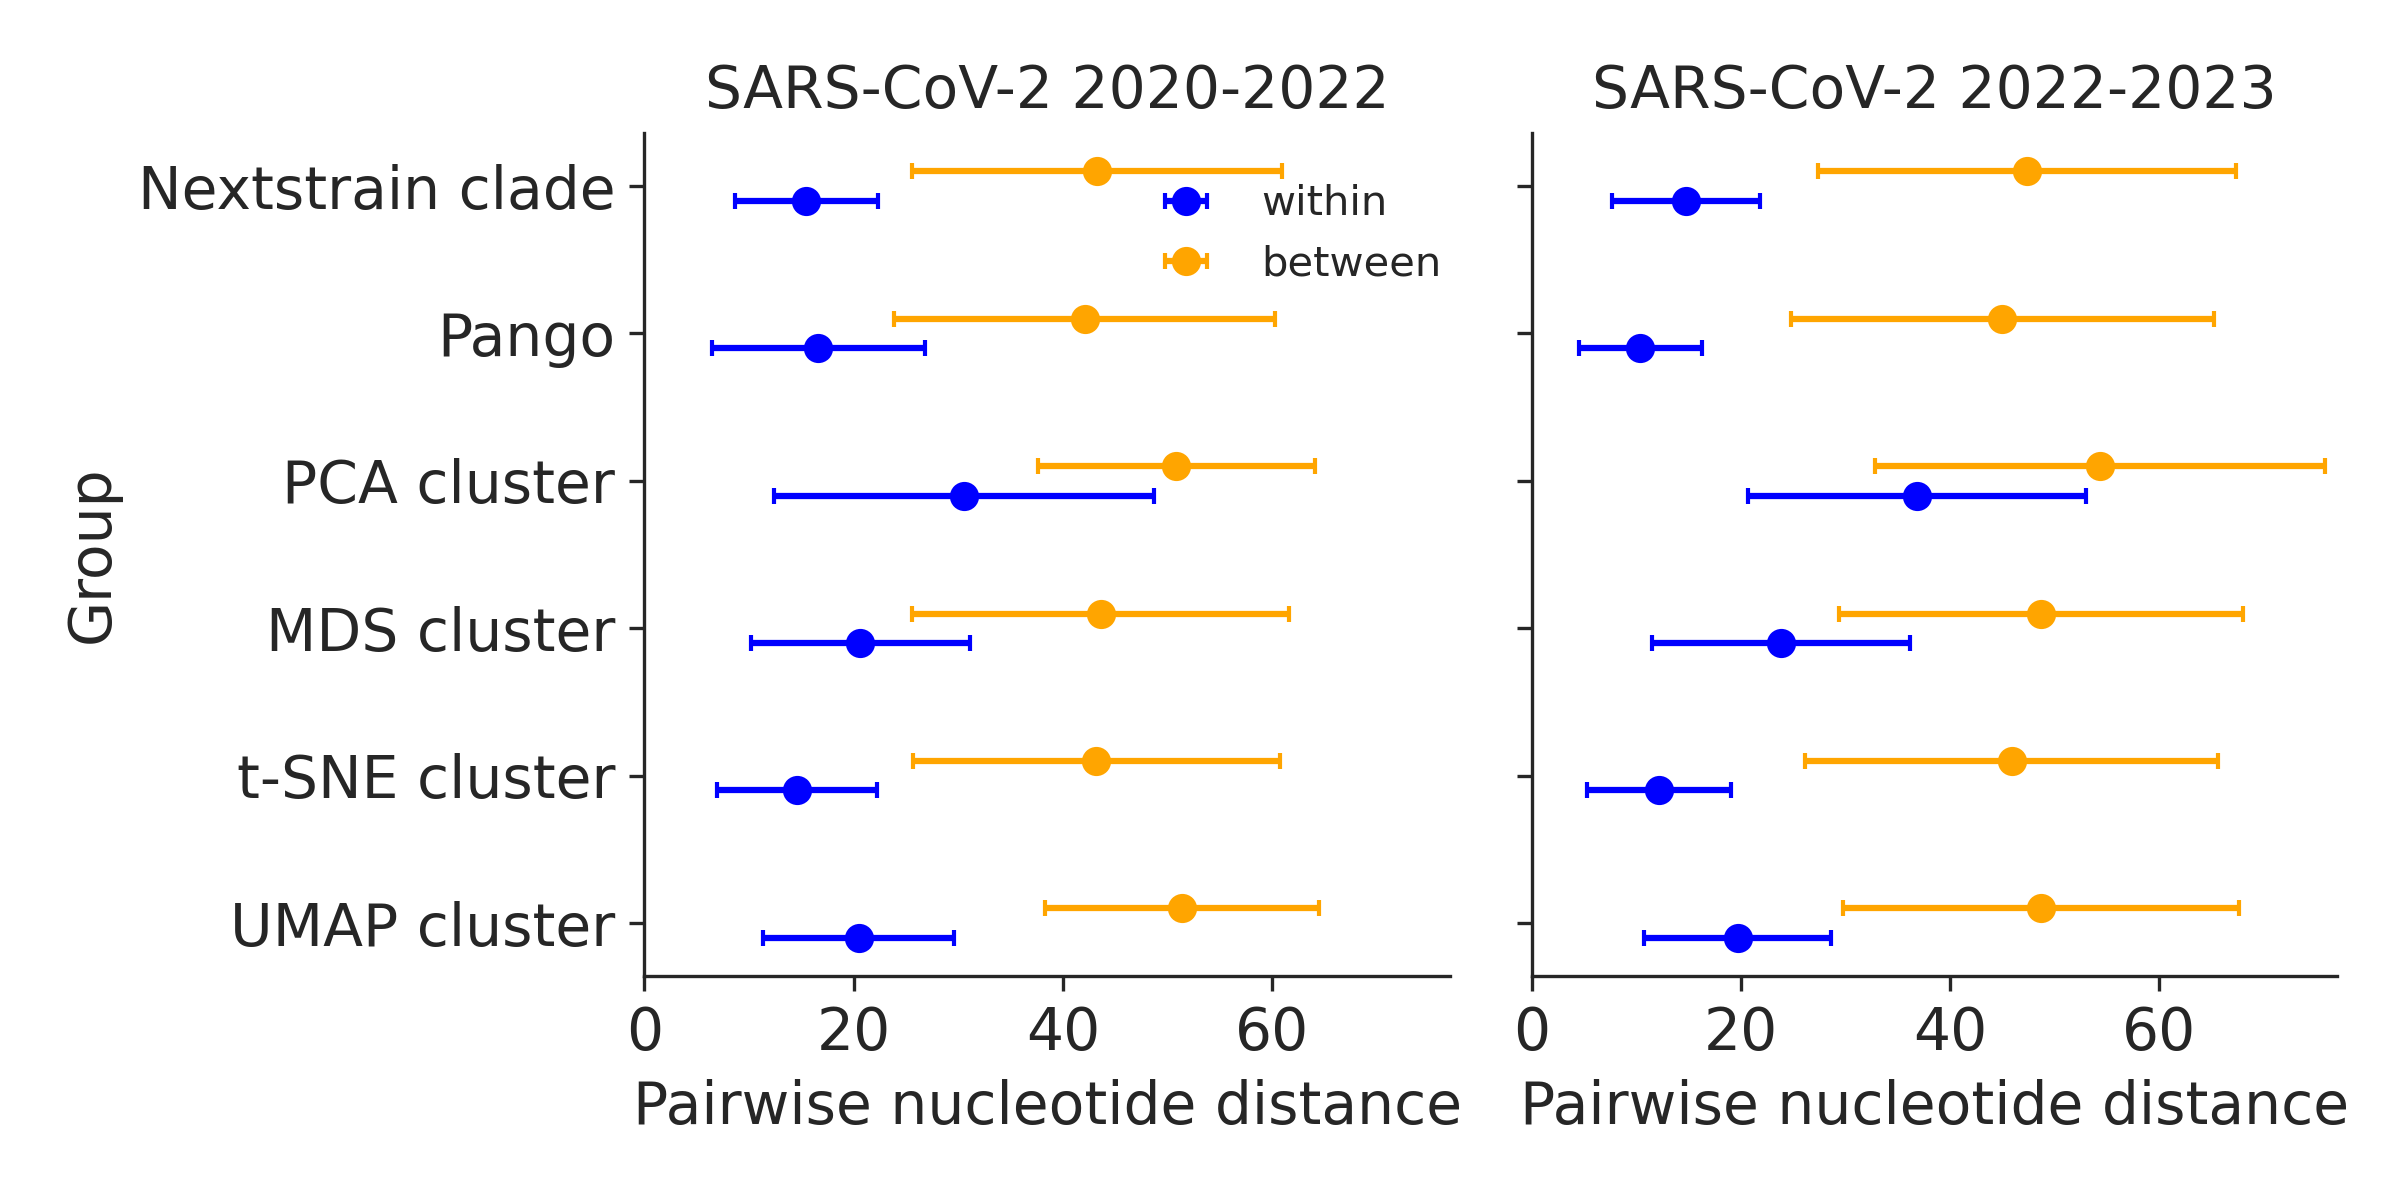
\includegraphics[width=\columnwidth]{figures/within_between_sars.png}
\caption{{\bf Pairwise nucleotide distances for early (2020-2022) and late (2022-2023) SARS-CoV-2 sequences within and between genetic groups defined by Nextstrain clades, Pango lineages, and clusters from PCA, MDS, t-SNE, and UMAP embeddings.}}\label{S_Fig_sarscov2_within_between_group_distances}
\end{figure}

\begin{figure}[!h]
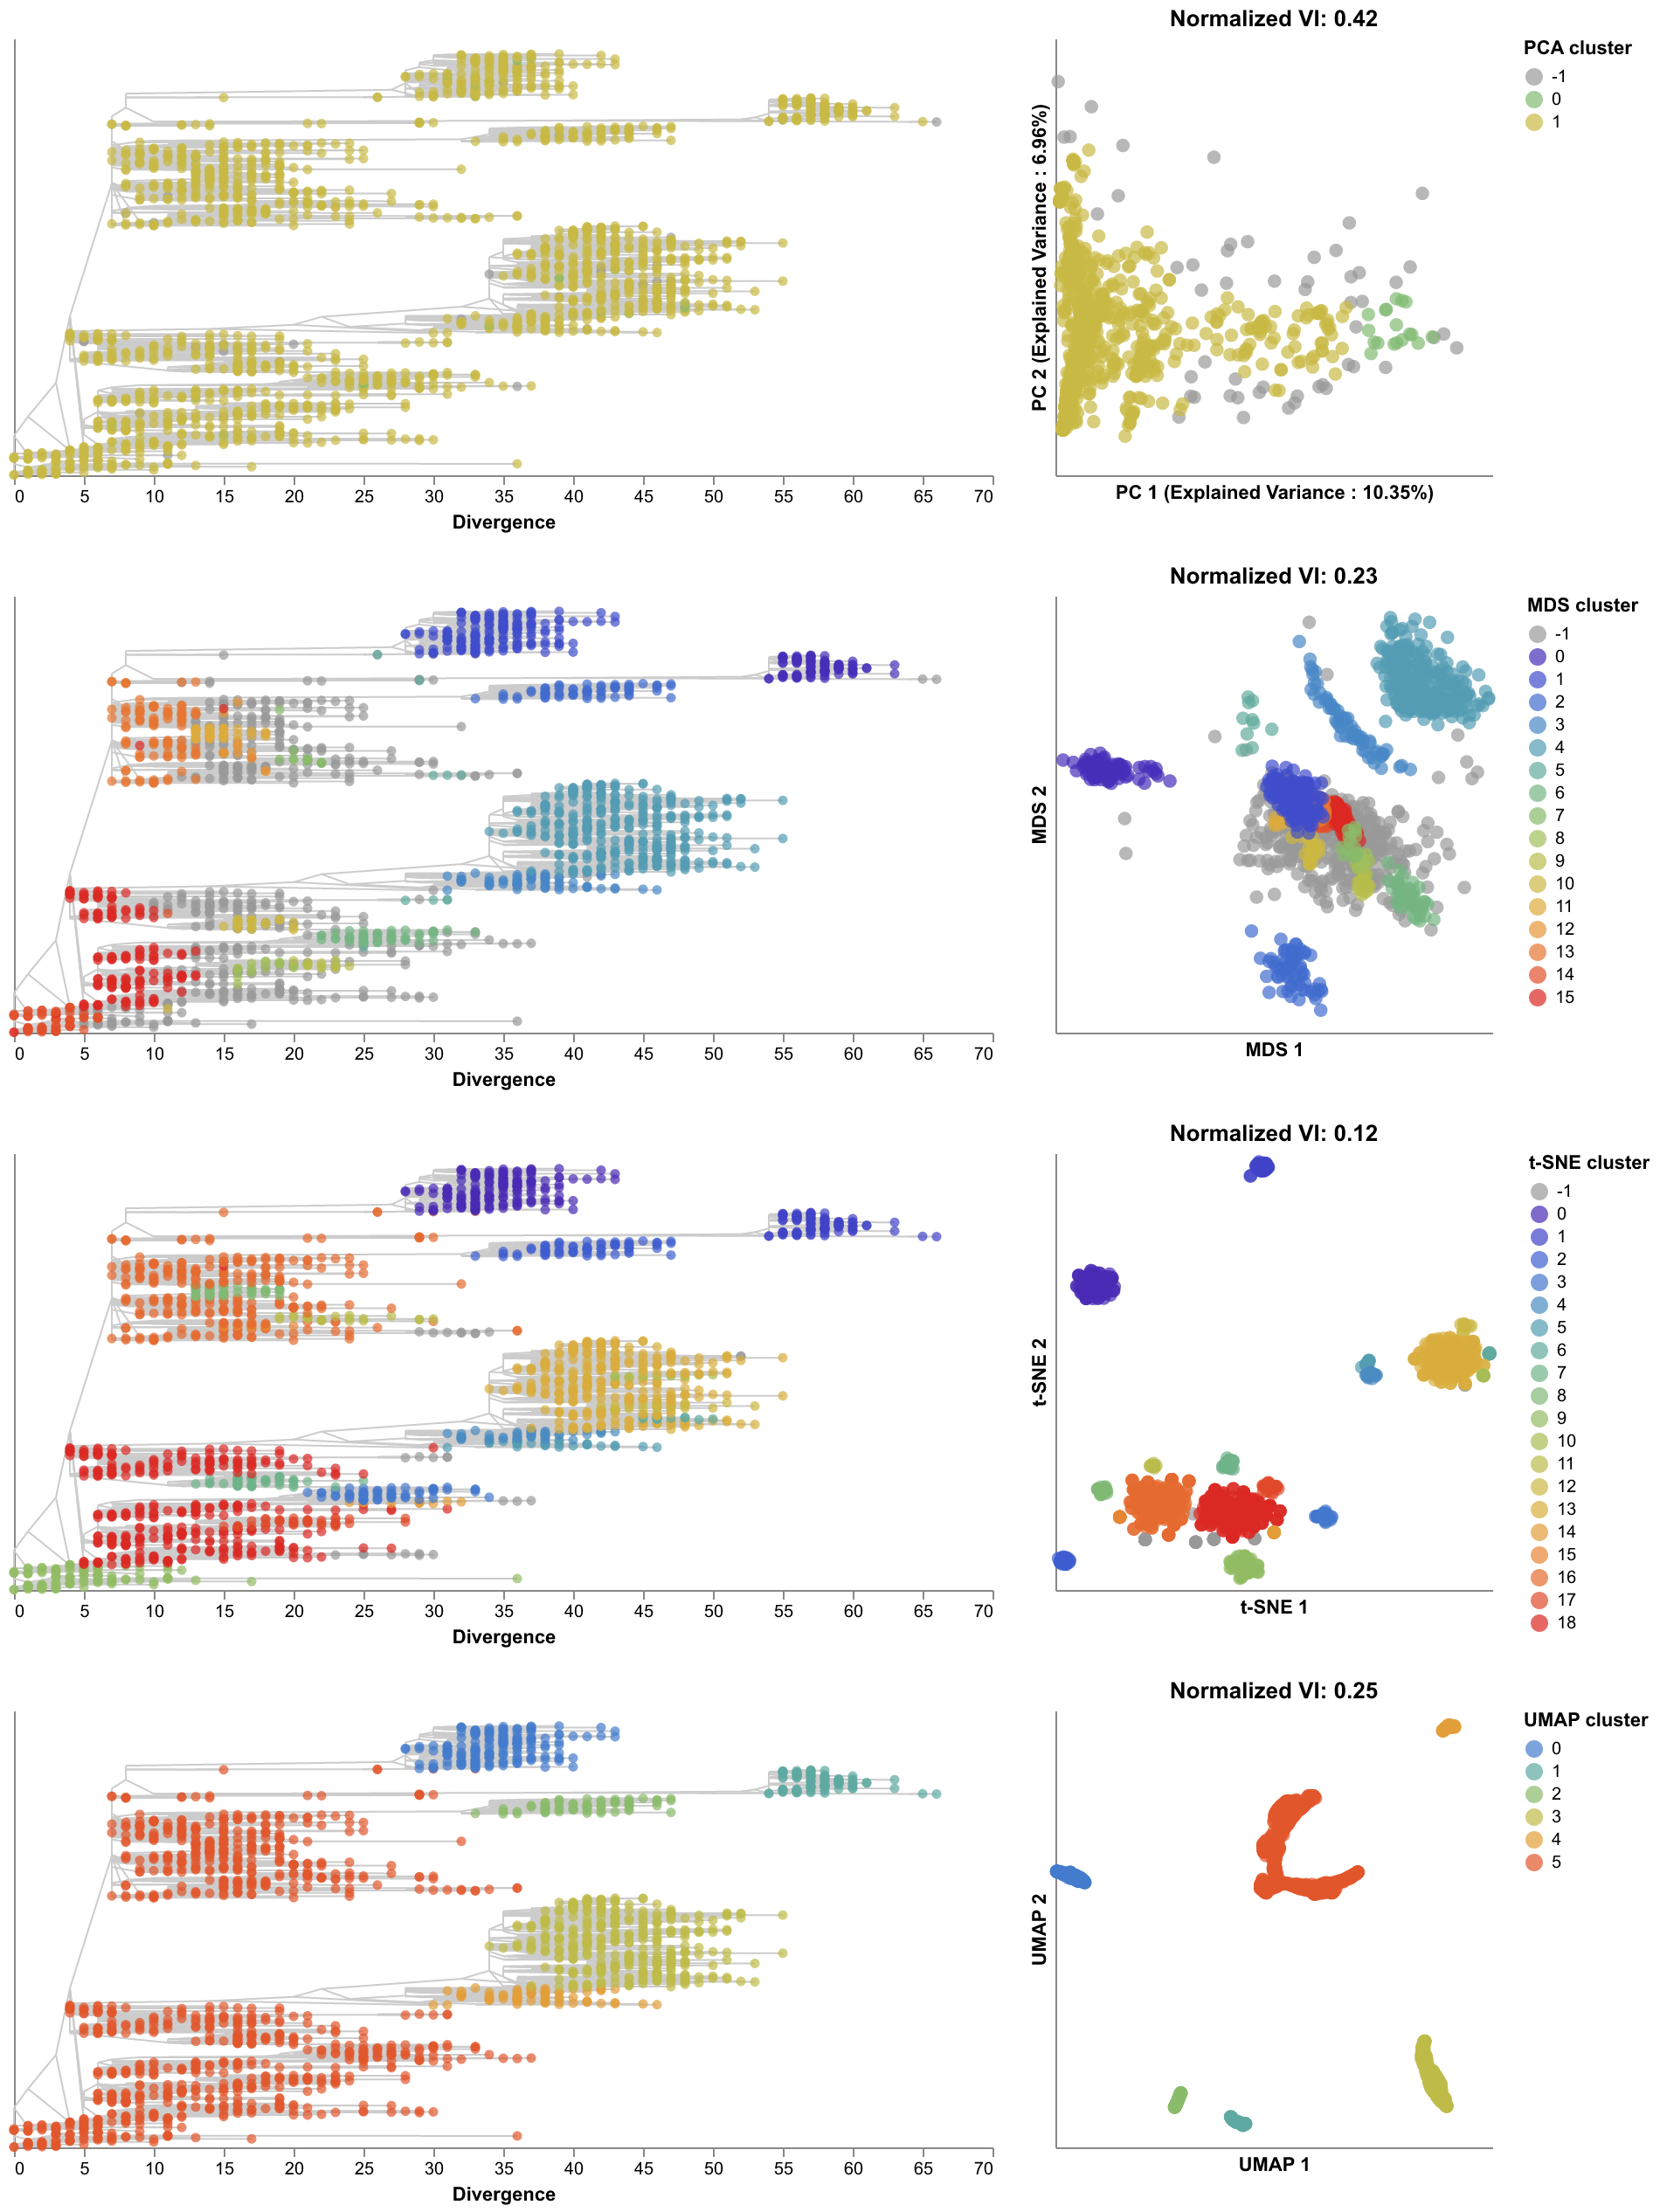
\includegraphics[width=\columnwidth]{figures/sarscov2-embeddings-by-cluster-vs-Nextclade_pango_collapsed.png}
\caption{{\bf Phylogenetic trees (left) and embeddings (right) of early (2020--2022) SARS-CoV-2 sequences colored by HDBSCAN cluster.}
  Normalized VI values per embedding reflect the distance between clusters and known genetic groups (Pango lineages).
  Line segments in each embedding reflect phylogenetic relationships with internal node positions calculated from the mean positions of their immediate descendants in each dimension (see Methods).
  Line thickness scales by the square root of the number of leaves descending from a given node in the phylogeny.
}\label{S_Fig_sarscov2_early_embeddings_by_cluster_vs_Nextclade_pango}
\end{figure}

\begin{figure}[!h]
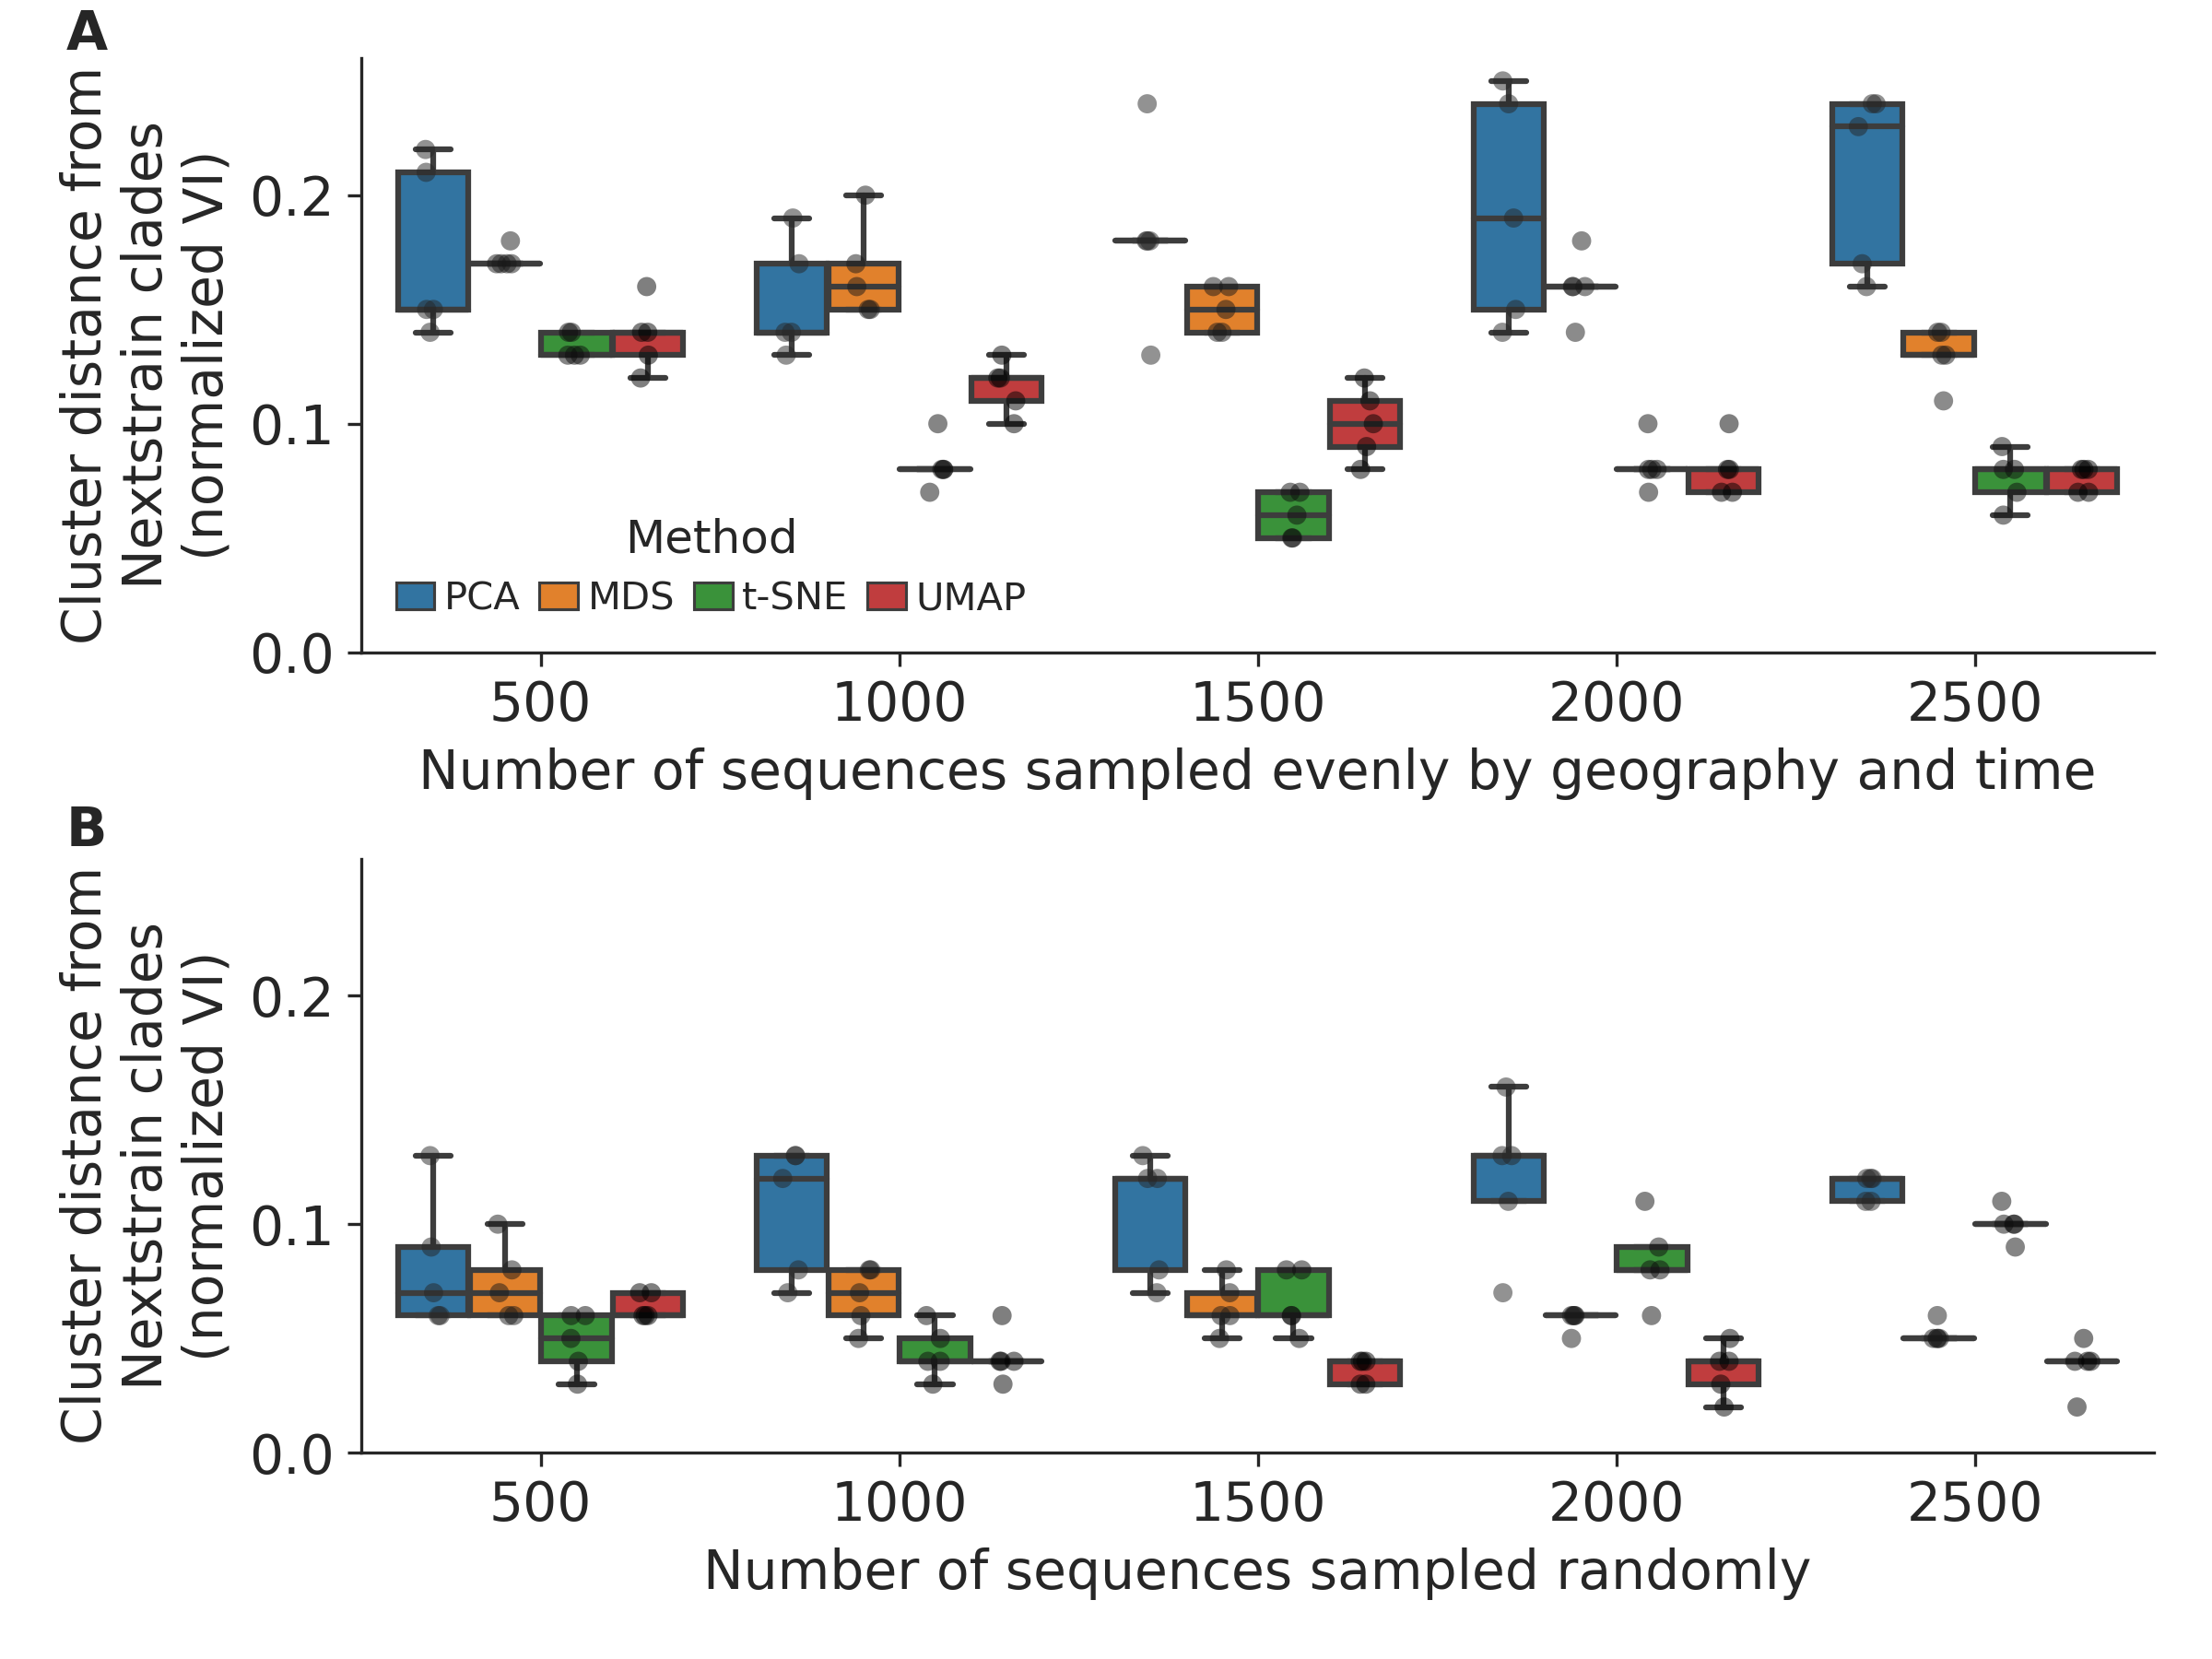
\includegraphics[width=\columnwidth]{figures/sarscov2-test-replication-of-cluster-accuracy.png}
\caption{{\bf Replication of cluster accuracy per embedding method for late (2022--2023) SARS-CoV-2 sequences across different sampling densities (total sequences sampled) and sampling schemes including A) even geographic and temporal sampling and B) random sampling.}
  We measured cluster accuracy across five replicates per sampling density and scheme with the normalized VI distance between clusters from a given embedding and Nextstrain clades for the same samples.
  The even sampling scheme selected sequences evenly across region, year, and month to minimize geographic and temporal bias.
  The random sampling scheme uniformly sampled from the original dataset, reflecting the geographic and genetic bias in those data.
}\label{S_Fig_late_sarscov2_replication_of_cluster_accuracy}
\end{figure}

\begin{figure}[!h]
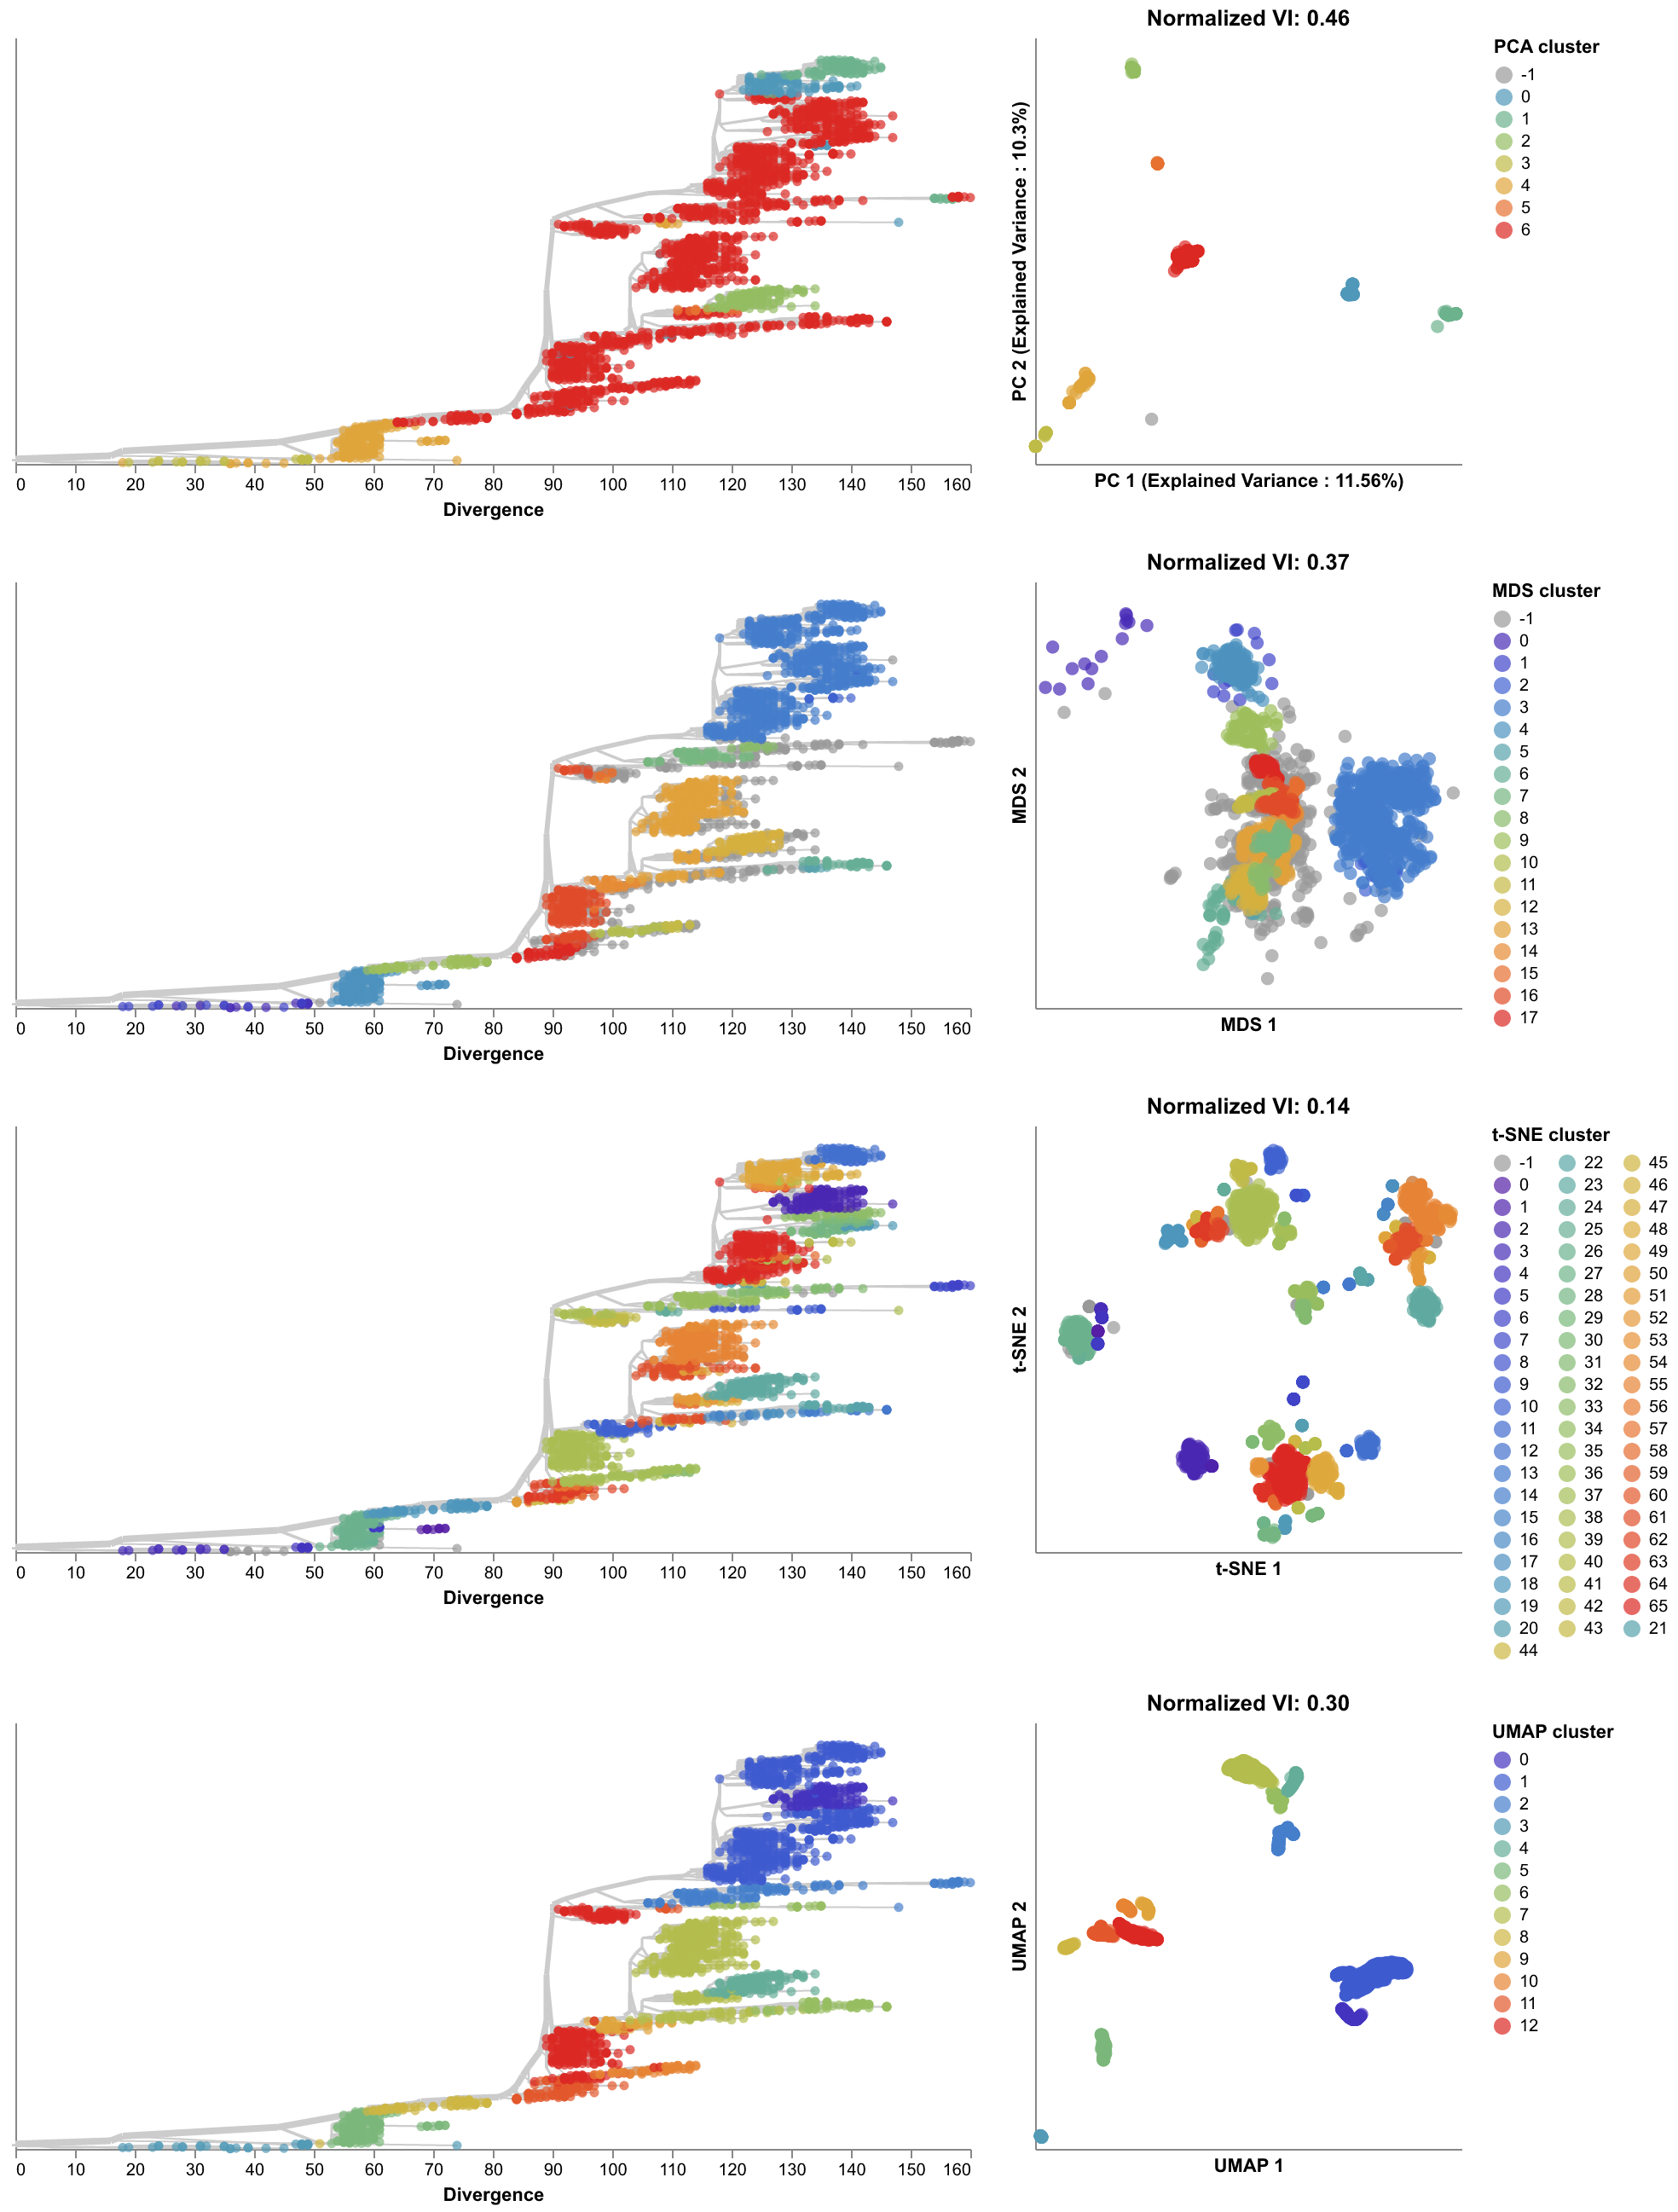
\includegraphics[width=\columnwidth]{figures/sarscov2-test-embeddings-by-cluster-vs-Nextclade_pango_collapsed.png}
\caption{{\bf Phylogenetic trees (left) and embeddings (right) of late (2022--2023) SARS-CoV-2 sequences colored by HDBSCAN cluster.}
  Normalized VI values per embedding reflect the distance between clusters and known genetic groups (Pango lineages).
}\label{S_Fig_sarscov2_late_embeddings_by_cluster_vs_Nextclade_pango}
\end{figure}

\begin{figure}[!h]
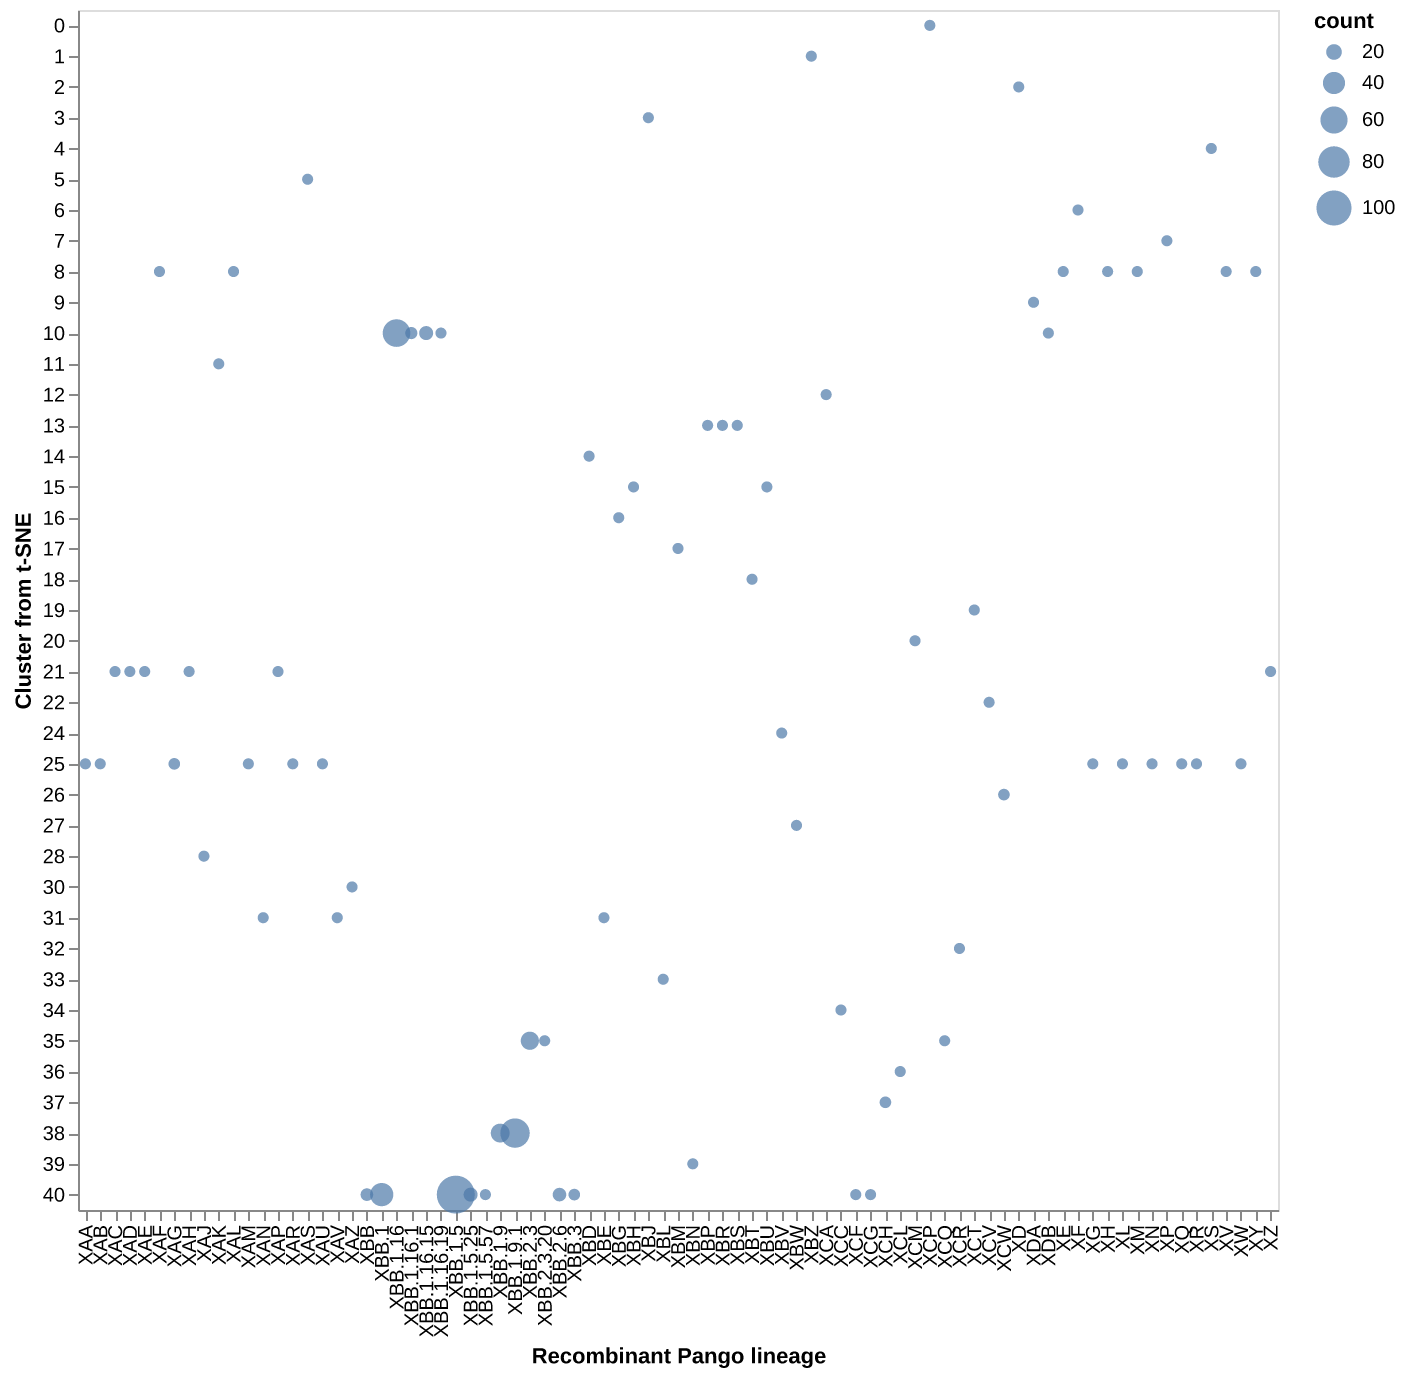
\includegraphics[width=\columnwidth]{figures/sarscov2-test-tsne-recombinant-counts-Nextstrain_clade.png}
\caption{{\bf Number of late SARS-CoV-2 strains per combination of recombinant Pango lineage and t-SNE cluster where the count was at least 10 strains.}}\label{S_Fig_sarscov2_late_embeddings_tsne_recombinant_counts}
\end{figure}
